\documentclass[13pt]{extarticle}

% ===================== GÓI LỆNH =====================
\usepackage[a4paper,top=3cm,bottom=2cm,left=3cm,right=2cm]{geometry}
\usepackage{fontspec}
\usepackage{polyglossia}
\setmainlanguage{vietnamese}
\setmainfont{Liberation Serif}
\setsansfont{Liberation Sans}
\setmonofont{DejaVu Sans Mono}[Scale=0.85]

\usepackage{setspace}
\onehalfspacing

\usepackage{titlesec}
\usepackage{tocloft}
\usepackage{graphicx}
\usepackage{float}
\usepackage{caption}
\usepackage{longtable}
\usepackage{array}
\usepackage{booktabs}
\usepackage{xcolor}
\usepackage{hyperref}
\usepackage{enumitem}
\usepackage{fancyhdr}
\usepackage{listings}
\usepackage{tikz}
\usetikzlibrary{shapes,arrows.meta,positioning,fit}

\hypersetup{
    colorlinks=true,
    linkcolor=black,
    urlcolor=blue,
    citecolor=black,
    pdftitle={Báo cáo Thực tập tốt nghiệp},
}

% ===================== ĐỊNH DẠNG TIÊU ĐỀ =====================
\titleformat{\section}{\normalfont\fontsize{15}{18}\bfseries}{PHẦN \thesection.}{0.5em}{}
\titleformat{\subsection}{\normalfont\fontsize{13}{16}\bfseries}{\thesubsection.}{0.5em}{}
\titleformat{\subsubsection}{\normalfont\fontsize{13}{16}\bfseries\itshape}{\thesubsubsection.}{0.5em}{}

\pagestyle{fancy}
\fancyhf{}
\fancyfoot[C]{\thepage}
\renewcommand{\headrulewidth}{0pt}

% ===================== LISTING CHO CODE =====================
\lstdefinestyle{javastyle}{
    language=Java,
    basicstyle=\ttfamily\small,
    keywordstyle=\color{blue}\bfseries,
    commentstyle=\color{gray}\itshape,
    stringstyle=\color{teal},
    numbers=left,
    numberstyle=\tiny\color{gray},
    breaklines=true,
    frame=single,
    backgroundcolor=\color{gray!5},
    tabsize=2,
}

% ===================== THÔNG TIN CÁ NHÂN =====================
\newcommand{\hoTenSV}{Bùi Minh Quân}
\newcommand{\maSV}{0212468}
\newcommand{\lopSV}{68CNCS}
\newcommand{\nganhSV}{Khoa học Máy tính}
\newcommand{\khoaVien}{Khoa Công nghệ Thông tin}
\newcommand{\gvhd}{Lê Văn Minh}
\newcommand{\mentorCT}{Nguyễn Gia Hưng}
\newcommand{\emailMentor}{hunggia@amazon.com.vn}
\newcommand{\donViThucTap}{Công ty TNHH Amazon Web Services Việt Nam -- Chương trình FCAJ (First Cloud AI Journey)}
\newcommand{\thoiGianTT}{25/07/2026 -- 08/09/2026}
\newcommand{\repositoryURL}{https://akaia1603.github.io/BuiMinhQuanWorkShopFCAJ/}

\begin{document}

% ===================== TRANG BÌA =====================
\begin{titlepage}
\centering
{\large BỘ GIÁO DỤC VÀ ĐÀO TẠO}\\
{\large\bfseries TRƯỜNG ĐẠI HỌC XÂY DỰNG HÀ NỘI}\\[0.3cm]
{\large \khoaVien}\\[2cm]

\rule{\linewidth}{0.5mm}\\[0.4cm]
{\huge\bfseries BÁO CÁO}\\[0.3cm]
{\Large\bfseries THỰC TẬP TỐT NGHIỆP}\\[0.4cm]
\rule{\linewidth}{0.5mm}\\[1cm]

{\large\bfseries Đề tài: Xây dựng Task Manager API trên nền tảng AWS Cloud\\ kết hợp Spring Boot Backend và Tích hợp AI}\\[2cm]

\begin{flushleft}
\large
\begin{tabular}{ll}
Sinh viên thực hiện: & \hoTenSV \\[0.2cm]
Mã số sinh viên: & \maSV \\[0.2cm]
Lớp: & \lopSV \\[0.2cm]
Ngành: & \nganhSV \\[0.2cm]
Giảng viên hướng dẫn tại trường: & \gvhd \\[0.2cm]
Cán bộ hướng dẫn tại đơn vị: & \mentorCT \\[0.2cm]
Đơn vị thực tập: & \donViThucTap \\[0.2cm]
Thời gian thực tập: & \thoiGianTT \\
\end{tabular}
\end{flushleft}

\vfill
{\large Hà Nội, 09/2026}

\end{titlepage}

% ===================== LỜI CẢM ƠN =====================
\section*{LỜI CẢM ƠN}
\addcontentsline{toc}{section}{LỜI CẢM ƠN}

Em xin bày tỏ lòng biết ơn chân thành nhất tới toàn thể thầy cô, các anh chị trong
chương trình thực tập đã giúp đỡ em trong quá trình hoàn thành báo cáo này.

Trước hết, em xin cảm ơn thầy \gvhd{} -- giảng viên hướng dẫn tại Khoa Công nghệ
Thông tin, Trường Đại học Xây dựng Hà Nội -- đã tận tình theo dõi, hướng dẫn em trong
suốt quá trình thực tập, giúp em định hướng nội dung kỹ thuật và kịp thời điều chỉnh
các vấn đề phát sinh.

Em xin cảm ơn Công ty TNHH Amazon Web Services Việt Nam và chương trình First Cloud AI
Journey (FCAJ) đã tạo điều kiện cho em được thực tập trong môi trường chuyên nghiệp,
cung cấp tài nguyên AWS Free Tier và tài liệu học tập phong phú. Đặc biệt, em xin
cảm ơn anh \mentorCT{} (\emailMentor) -- cán bộ hướng dẫn tại đơn vị thực tập
-- đã luôn đồng hành, hỗ trợ em trong các quyết định kiến trúc, review tiến độ và
khuyến khích em tự tìm hiểu giải pháp trước khi nhờ hỗ trợ.

Em cũng xin cảm ơn gia đình và bạn bè đã luôn động viên, hỗ trợ em trong suốt thời
gian thực tập và viết báo cáo.

\newpage

% ===================== MỤC LỤC =====================
\tableofcontents
\newpage

% ===================== DANH MỤC HÌNH, BẢNG, TỪ VIẾT TẮT =====================
\listoffigures
\addcontentsline{toc}{section}{DANH MỤC HÌNH VẼ}
\newpage

\listoftables
\addcontentsline{toc}{section}{DANH MỤC BẢNG BIỂU}
\newpage

\section*{DANH MỤC TỪ VIẾT TẮT}
\addcontentsline{toc}{section}{DANH MỤC TỪ VIẾT TẮT}
\begin{longtable}{p{3cm}p{11cm}}
\toprule
\textbf{Từ viết tắt} & \textbf{Giải nghĩa} \\
\midrule
\endhead
TTTN & Thực tập tốt nghiệp \\
FCAJ & First Cloud AI Journey (chương trình thực tập AWS Cloud) \\
AWS & Amazon Web Services \\
EC2 & Elastic Compute Cloud \\
RDS & Relational Database Service \\
S3 & Simple Storage Service \\
VPC & Virtual Private Cloud \\
CLO & Course Learning Outcome (Chuẩn đầu ra học phần) \\
API & Application Programming Interface \\
JWT & JSON Web Token \\
CRUD & Create, Read, Update, Delete \\
IAM & Identity and Access Management \\
CI/CD & Continuous Integration / Continuous Deployment \\
CDN & Content Delivery Network \\
NLP & Natural Language Processing \\
\bottomrule
\end{longtable}
\newpage

% ===================== PHẦN 1 =====================
\section{GIỚI THIỆU CHUNG VỀ ĐƠN VỊ THỰC TẬP}

\subsection{Giới thiệu chương trình thực tập}

Chương trình First Cloud AI Journey (FCAJ) là chương trình thực tập trực tuyến
định hướng công nghệ đám mây, do Công ty TNHH Amazon Web Services Việt Nam tổ chức
tại \url{https://cloudjourney.awsstudygroup.com/}. Chương trình được thiết kế theo mô
hình học qua thực hành (learning-by-doing): sinh viên hoàn thành khóa học nền tảng
về AWS Cloud, sau đó triển khai một chuỗi các workshop thực hành nhỏ và một dự án
ứng dụng hoàn chỉnh nhằm chứng minh năng lực vận dụng kiến thức vào giải quyết bài
toán thực tế.

Chương trình FCAJ kéo dài 7 tuần, bắt đầu bằng việc định hướng giới thiệu công ty,
tạo tài khoản AWS và khám phá các dịch vụ đám mây cốt lõi. Qua từng tuần, sinh viên
đi sâu vào các nhóm dịch vụ Compute (EC2), Storage (S3), Networking (VPC), Serverless
(Lambda, API Gateway, DynamoDB), Database (RDS), và giám sát chi phí (Budgets,
CloudWatch), trước khi xây dựng dự án chính -- một ứng dụng backend hoàn chỉnh
triển khai trên hạ tầng AWS thật.

\subsection{Lĩnh vực hoạt động liên quan đến chuyên môn}

Nội dung thực tập tập trung vào hai mảng kỹ thuật chính, phù hợp với định
hướng nghề nghiệp Java Backend Developer của sinh viên. Mảng thứ nhất là
\textbf{điện toán đám mây (Cloud Computing)}, theo đó sinh viên làm quen và
thực hành các dịch vụ nền tảng của AWS trải dài từ Compute (EC2), Storage
(S3), Networking (VPC), Serverless (Lambda, API Gateway, DynamoDB), Database
(RDS), CDN (CloudFront) cho tới giám sát chi phí (Budgets, CloudWatch). Mảng
thứ hai là \textbf{phát triển Backend bằng Java/Spring Boot}, tập trung vào
việc xây dựng REST API, xác thực bằng JWT, thiết kế cơ sở dữ liệu quan hệ,
triển khai ứng dụng theo mô hình client-server trên hạ tầng cloud thật, và
tích hợp dịch vụ AI (Amazon Comprehend) vào ứng dụng.

\subsection{Bối cảnh và lý do lựa chọn nội dung thực tập}

Sinh viên là sinh viên năm cuối ngành Khoa học Máy tính (lớp 68CNCS), đang chuẩn bị bước
vào lĩnh vực phát triển phần mềm Backend theo hướng Java. Việc kết hợp thực
hành AWS Cloud với một dự án Backend Java thực tế giúp sinh viên vừa đáp ứng
yêu cầu của chương trình FCAJ, vừa xây dựng được portfolio kỹ thuật sát với
định hướng tuyển dụng thực tế của ngành công nghiệp phần mềm hiện nay, nơi kỹ
năng triển khai ứng dụng lên hạ tầng cloud là một yêu cầu phổ biến đối với vị
trí Backend Developer.

Đặc biệt, dự án được mở rộng tích hợp AI (Amazon Comprehend) để đáp ứng CLO3
(vận dụng kiến thức AI vào bài toán thực tế), giúp sinh viên không chỉ dừng lại ở
phát triển Backend thông thường mà còn có kinh nghiệm nhúng dịch vụ AI vào ứng dụng
thực tế -- một kỹ năng ngày càng quan trọng trong xu hướng phát triển phần mềm hiện nay.

\newpage

% ===================== PHẦN 2 =====================
\section{MỤC TIÊU VÀ KẾ HOẠCH THỰC TẬP}

\subsection{Mục tiêu học tập cá nhân theo chuẩn đầu ra (CLO)}

Theo đề cương chi tiết học phần Thực tập tốt nghiệp của Khoa Công nghệ Thông
tin áp dụng cho hệ Cử nhân (3 tín chỉ), học phần có 5 chuẩn đầu ra (CLO).
Bảng \ref{tab:clo-goals} trình bày mục tiêu cụ thể của sinh viên đối với
từng CLO trong đợt thực tập này.

\begin{longtable}{p{1.5cm}p{5cm}p{7.5cm}}
\caption{Mục tiêu học tập cá nhân theo từng CLO}
\label{tab:clo-goals} \\
\toprule
\textbf{CLO} & \textbf{Mô tả chuẩn đầu ra} & \textbf{Mục tiêu cụ thể trong đợt thực tập} \\
\midrule
\endhead
CLO1 & Phân tích nội dung, đặc điểm và phạm vi ứng dụng của giải pháp công
nghệ đã tiếp cận trong giai đoạn thực tập &
Phân tích được kiến trúc và đặc điểm kỹ thuật của các dịch vụ AWS (S3,
CloudFront, Lambda, API Gateway, DynamoDB, VPC, EC2, RDS, Comprehend) và phạm vi ứng dụng
của từng dịch vụ trong hệ thống backend thực tế. \\
CLO2 & Thiết kế được giải pháp kỹ thuật có tính khả thi và ứng dụng thực tế
&
Thiết kế và triển khai được một REST API hoàn chỉnh (Task Manager API) chạy
trên kiến trúc EC2 + RDS trong VPC 2-tier, giải quyết bài toán quản lý công việc/dự án nhỏ,
kết hợp tích hợp AI tự động gợi ý mức ưu tiên task. \\
CLO3 & Vận dụng kiến thức về trí tuệ nhân tạo để triển khai một bài toán
Khoa học Máy tính trong môi trường thực tế &
Tích hợp Amazon Comprehend (dịch vụ AI/NLP của AWS) vào Task Manager API để
tự động phân tích sentiment và trích xuất từ khóa từ mô tả công việc, qua đó
gợi ý mức độ ưu tiên (Priority) cho từng task -- ứng dụng AI giải quyết bài
toán thực tế trong hệ thống quản lý công việc. \\
CLO4 & Giao tiếp hiệu quả bằng hình thức viết và nói trong môi trường công
việc &
Viết đầy đủ Worklog cho từng tuần, Blog kỹ thuật (Blog về Guardrails trong Amazon Bedrock Knowledge Bases),
bài thu hoạch sự kiện (AWS Vietnam Community Meetup), và trình bày báo cáo
thực tập rõ ràng, có cấu trúc. \\
CLO5 & Làm việc nhóm hiệu quả trong môi trường thực tế, chuyên nghiệp &
Trao đổi thường xuyên với giảng viên hướng dẫn (\gvhd) và mentor công ty
(\mentorCT) để định hướng nội dung kỹ thuật, tuân thủ deadline và quy trình
báo cáo của chương trình FCAJ. \\
\bottomrule
\end{longtable}

\subsection{Kế hoạch công việc chi tiết}

Do học phần thuộc hệ Cử nhân với khối lượng 3 tín chỉ, kế hoạch được rút gọn
so với chương trình Kỹ sư, tập trung vào việc hoàn thành các workshop nền tảng
song song với dự án chính. Bảng \ref{tab:plan} trình bày kế hoạch triển khai
theo tuần, khớp với Phiếu theo dõi tiến độ thực tập đã được phê duyệt.

\begin{longtable}{p{1.8cm}p{12cm}}
\caption{Kế hoạch công việc theo tuần}
\label{tab:plan} \\
\toprule
\textbf{Thời gian} & \textbf{Nội dung công việc} \\
\midrule
\endhead
Tuần 1 & (25/07--31/07) Nghe giới thiệu về công ty, nhân sự và đối tác liên kết;
tạo tài khoản AWS Free Tier; thiết lập MFA và cảnh báo chi phí; khám phá AWS
Management Console và các nhóm dịch vụ chính (Compute, Storage, Networking, Database). \\
Tuần 2 & (01/08--07/08) Học và thực hành EC2 (loại instance, AMI, EBS volume, Security
Group); lab khởi chạy EC2 và kết nối SSH; học VPC (subnet, route table, Internet
Gateway, CIDR); lab tạo VPC tùy chỉnh với public subnet và triển khai ứng dụng
web đơn giản trên EC2. \\
Tuần 3 & (08/08--14/08) Học S3 storage class, versioning, lifecycle policy; thực hành
DynamoDB (tạo bảng, insert/query qua console và CLI); cấu hình S3 versioning và khôi phục
object; học CloudWatch (metrics, alarm, logs, dashboard) và tạo alarm cho CPU
utilization; cài đặt AWS CLI và quản lý tài nguyên qua dòng lệnh. \\
Tuần 4 & (15/08--21/08) Thiết lập AWS Budget (\texttt{FCAJ-Budget}, 5 USD/tháng) và
CloudWatch billing alarm; triển khai Workshop Static Website (S3 + CloudFront
với HTTPS); triển khai Workshop Serverless Notes API (Lambda + API Gateway +
DynamoDB); kiểm thử GET/POST qua Postman. \\
Tuần 5 & (22/08--28/08) Thiết kế VPC 2-tier (public/private subnet, 2 AZ); khởi
chạy EC2 trong public subnet và kiểm thử SSH; thiết kế database Task Manager
(users/projects/tasks); cấp phát RDS MySQL private (Free tier, \texttt{db.t3.micro});
triển khai backend Spring Boot trên EC2 dưới dạng systemd service; kiểm thử
JWT register. \\
Tuần 6 & (29/08--04/09) Tạo IAM Role \texttt{taskmanager-ec2-comprehend-role} với
policy \texttt{ComprehendReadOnly}; gắn role vào EC2 và tích hợp Amazon Comprehend;
triển khai frontend lên EC2 với Nginx; kiểm thử end-to-end qua trình duyệt
(JWT auth, CRUD project/task, AI priority); ghi hướng dẫn dọn dẹp tài nguyên. \\
Tuần 7 & (05/09--08/09) Fork template Hugo, tùy chỉnh config.toml; điền nội dung
worklog, proposal, workshop; cấu hình GitHub Actions deploy lên GitHub Pages;
viết phần tự đánh giá, phản hồi và bài thu hoạch sự kiện; đọc soát và nộp báo cáo. \\
\bottomrule
\end{longtable}

\newpage

% ===================== PHẦN 3 =====================
\section{NỘI DUNG VÀ KẾT QUẢ THỰC TẬP: WORKSHOP AWS CLOUD}

Phần này trình bày toàn bộ nội dung thực hành đã triển khai trong đợt thực
tập, theo trình tự từ chuẩn bị môi trường, các workshop nền tảng, cho tới
dự án chính -- Task Manager API tích hợp AI. Mỗi mục đều ghi rõ các bước
thao tác trên AWS Console kèm ảnh minh chứng.

\subsection{Chuẩn bị môi trường và thiết lập Region}

\subsubsection{Yêu cầu tiên quyết}

Để thực hiện các bước dưới đây, sinh viên cần chuẩn bị sẵn một tài khoản AWS
Free Tier có quyền quản trị (Root account) hoặc IAM User có đủ quyền thao tác
trên các dịch vụ S3, CloudFront, Lambda, API Gateway, DynamoDB, VPC, EC2, RDS,
Comprehend, Budgets, CloudWatch và IAM; một trình duyệt web chạy tốt (Chrome,
Firefox, Edge); công cụ kiểm thử API là Postman hoặc curl; cùng với JDK 17,
Maven và Docker cài trên máy cá nhân để build và test trước khi triển khai
lên EC2.

\subsubsection{Các bước thực hiện}

\begin{enumerate}[leftmargin=1.5cm]
    \item Truy cập \url{https://console.aws.amazon.com} và đăng nhập tài
    khoản AWS đã tạo ở Tuần 1.

    \begin{figure}[H]
        \centering
        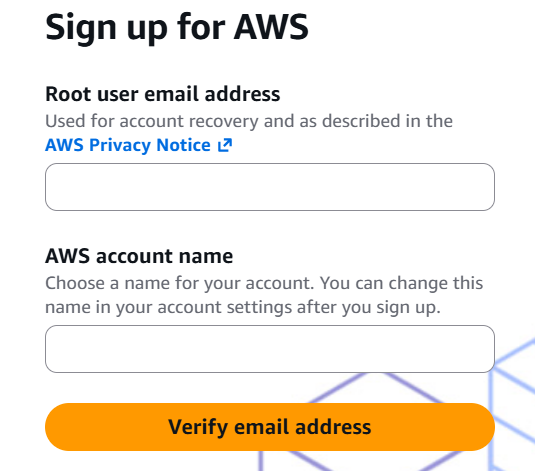
\includegraphics[width=12cm]{static/images/5-Workshop/5.2-Environment-Setup/01-console-login.png}
        \caption{Trang đăng nhập AWS Console}
        \label{fig:console-login}
    \end{figure}

    \item Ở góc trên bên phải thanh điều hướng, chọn Region
    \textbf{Asia Pacific (Singapore) -- ap-southeast-1}. Toàn bộ dịch vụ trong
    báo cáo này đều triển khai cùng một region để tránh lỗi kết nối chéo vùng.

    \begin{figure}[H]
        \centering
        
\includegraphics[width=12cm]{static/images/5-Workshop/5.2-Environment-Setup/02-region-selector.png}
        \caption{Chọn Region ap-southeast-1 từ góc trên bên phải Console}
        \label{fig:region-selector}
    \end{figure}

    \item Xác nhận Region đã chọn đúng -- góc trên bên phải hiển thị ``Asia Pacific
    (Singapore)''.

    \begin{figure}[H]
        \centering
        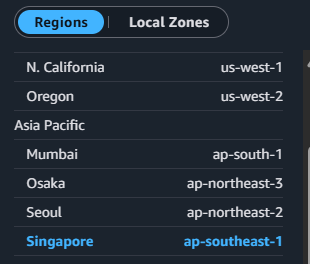
\includegraphics[width=12cm]{static/images/5-Workshop/5.2-Environment-Setup/03-region-confirmed.png}
        \caption{Console sau khi đã chuyển đúng Region}
        \label{fig:region-confirmed}
    \end{figure}
\end{enumerate}

\subsection{Giám sát và kiểm soát chi phí (AWS Budgets \& CloudWatch)}

Trước khi triển khai bất kỳ dịch vụ nào phát sinh chi phí, sinh viên thiết
lập cơ chế giám sát để đảm bảo không vượt ngưỡng Free Tier.

\subsubsection{Tạo AWS Budget}

\begin{enumerate}[leftmargin=1.5cm]
    \item Tại thanh tìm kiếm, gõ \textbf{Budgets} → chọn AWS Budgets →
    \textbf{Create budget}.

    \begin{figure}[H]
        \centering
        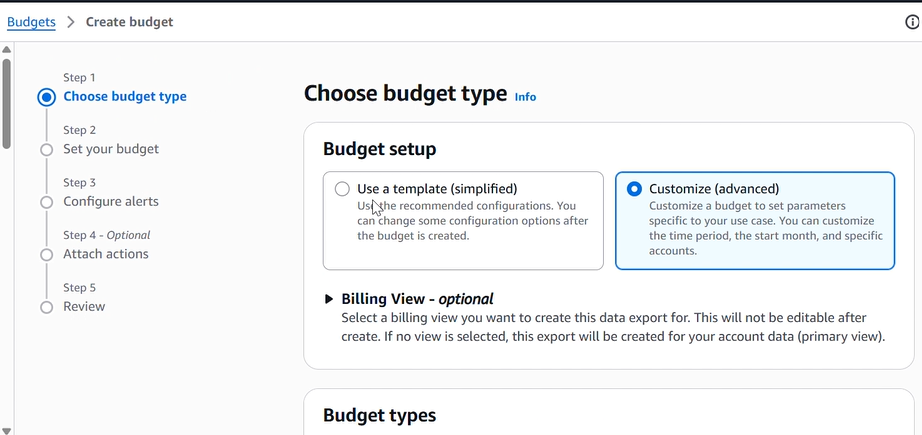
\includegraphics[width=10cm]{static/images/5-Workshop/5.3-Cost-Monitoring/01-budget-menu.png}
        \caption{Trang AWS Budgets}
        \label{fig:budget-menu}
    \end{figure}

    \item Chọn \textit{Customize (advanced)} → Cost budget → đặt tên
    \texttt{FCAJ-Budget}, Period: Monthly, Budgeted amount: 5 USD.

    \begin{figure}[H]
        \centering
        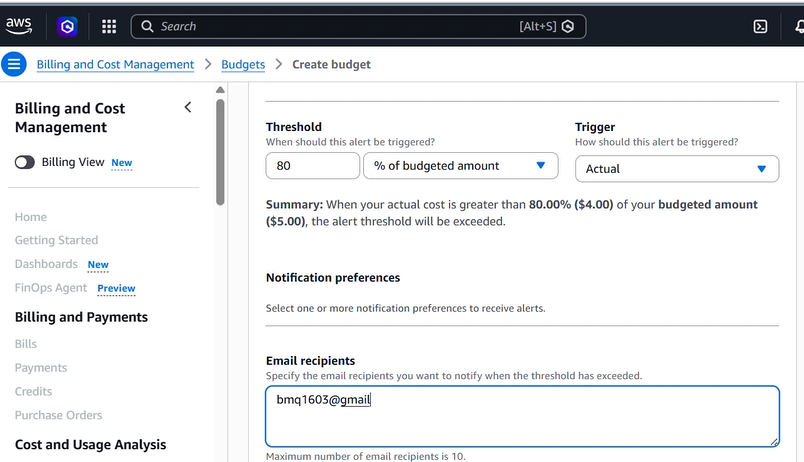
\includegraphics[width=10cm]{static/images/5-Workshop/5.3-Cost-Monitoring/02-budget-create.png}
        \caption{Cấu hình tạo Budget: \texttt{FCAJ-Budget}, Monthly, 5 USD}
        \label{fig:budget-create}
    \end{figure}

    \item Thêm 2 ngưỡng cảnh báo (Alert threshold) tại 50\% và 80\%, nhập
    email nhận thông báo → \textbf{Create budget}.

    \begin{figure}[H]
        \centering
        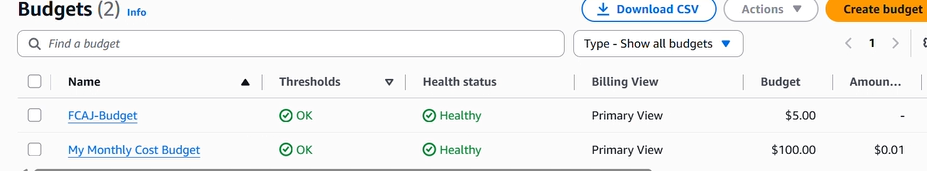
\includegraphics[width=10cm]{static/images/5-Workshop/5.3-Cost-Monitoring/03-budget-list.png}
        \caption{Danh sách Budget hiển thị \texttt{FCAJ-Budget}}
        \label{fig:budget-list}
    \end{figure}
\end{enumerate}

\subsubsection{Bật Billing Alerts và tạo CloudWatch Alarm}

\begin{enumerate}[leftmargin=1.5cm]
    \item Chuyển Region sang \textbf{us-east-1 (N. Virginia)}, vào Billing
    Preferences, bật \textit{Receive Billing Alerts}.

    \begin{figure}[H]
        \centering
        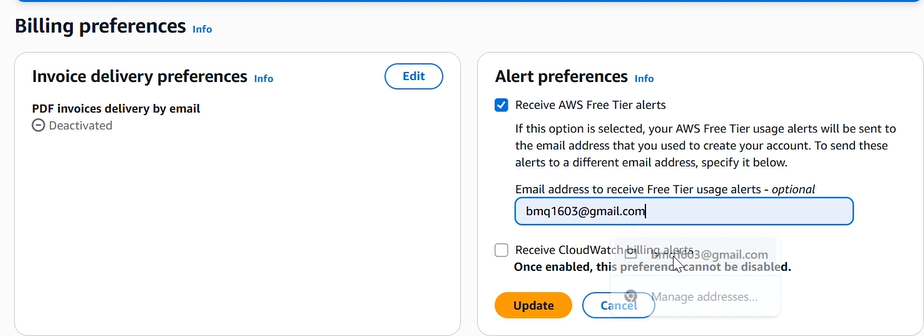
\includegraphics[width=10cm]{static/images/5-Workshop/5.3-Cost-Monitoring/04-billing-preferences.png}
        \caption{Billing Preferences -- Receive Billing Alerts đã bật}
        \label{fig:billing-prefs}
    \end{figure}

    \item Vào CloudWatch → Alarms → Billing → \textbf{Create alarm}, chọn
    metric \texttt{EstimatedCharges}, ngưỡng > 5 USD, tạo SNS topic gửi
    email cảnh báo.

    \begin{figure}[H]
        \centering
        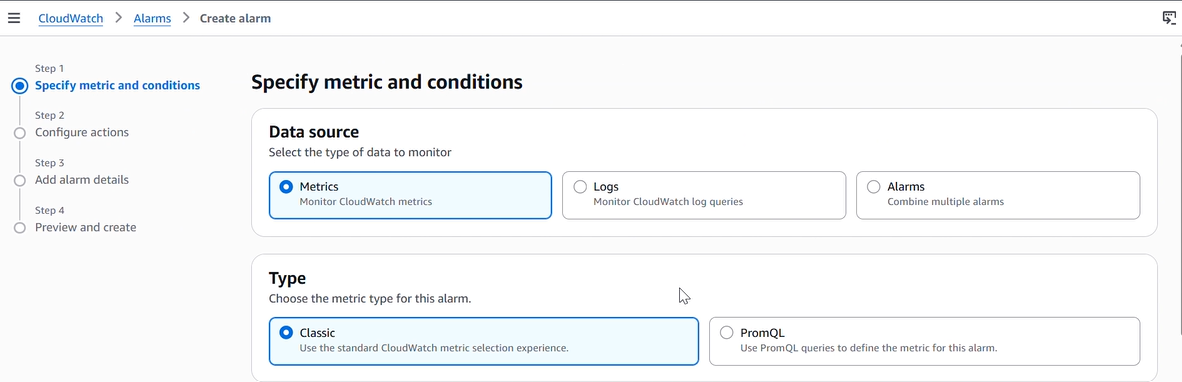
\includegraphics[width=10cm]{static/images/5-Workshop/5.3-Cost-Monitoring/05-cloudwatch-alarm-create.png}
        \caption{Tạo CloudWatch Billing Alarm trên metric \texttt{EstimatedCharges}}
        \label{fig:cw-alarm-create}
    \end{figure}

    \begin{figure}[H]
        \centering
        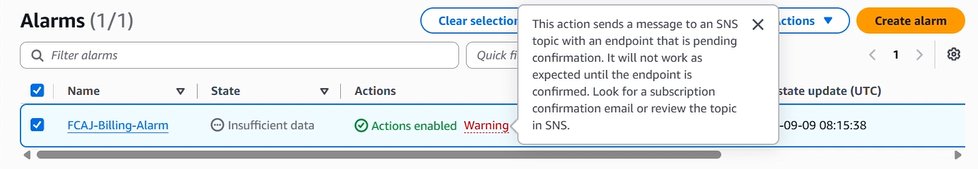
\includegraphics[width=10cm]{static/images/5-Workshop/5.3-Cost-Monitoring/06-cloudwatch-alarm-ok.png}
        \caption{Billing Alarm ở trạng thái ``OK''}
        \label{fig:cw-alarm-ok}
    \end{figure}

    \item Kiểm tra email xác nhận subscription từ AWS Notifications.

    \begin{figure}[H]
        \centering
        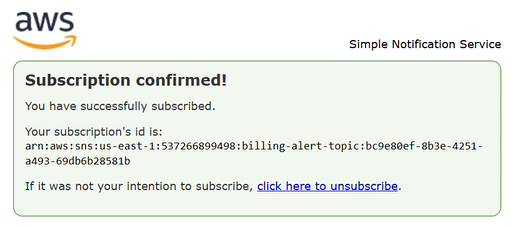
\includegraphics[width=10cm]{static/images/5-Workshop/5.3-Cost-Monitoring/07-subscription-email.png}
        \caption{Email xác nhận subscription từ AWS Notifications}
        \label{fig:subscription-email}
    \end{figure}
\end{enumerate}

\subsection{Triển khai Website tĩnh (S3 + CloudFront)}

Workshop này xây dựng một website tĩnh được host trên S3 và phục vụ qua CloudFront
bằng giao thức HTTPS -- mô hình thường dùng cho frontend của các ứng dụng web hiện đại.

Sơ đồ kiến trúc: Người dùng $\rightarrow$ CloudFront (CDN, HTTPS) $\rightarrow$ S3 Bucket
(chứa file HTML/CSS/JS tĩnh).

\begin{enumerate}[leftmargin=1.5cm]
    \item Tạo S3 bucket (tên duy nhất toàn cầu), region \texttt{ap-southeast-1}.
    Bỏ tick \textit{Block all public access} để cho phép truy cập công khai.

    \begin{figure}[H]
        \centering
        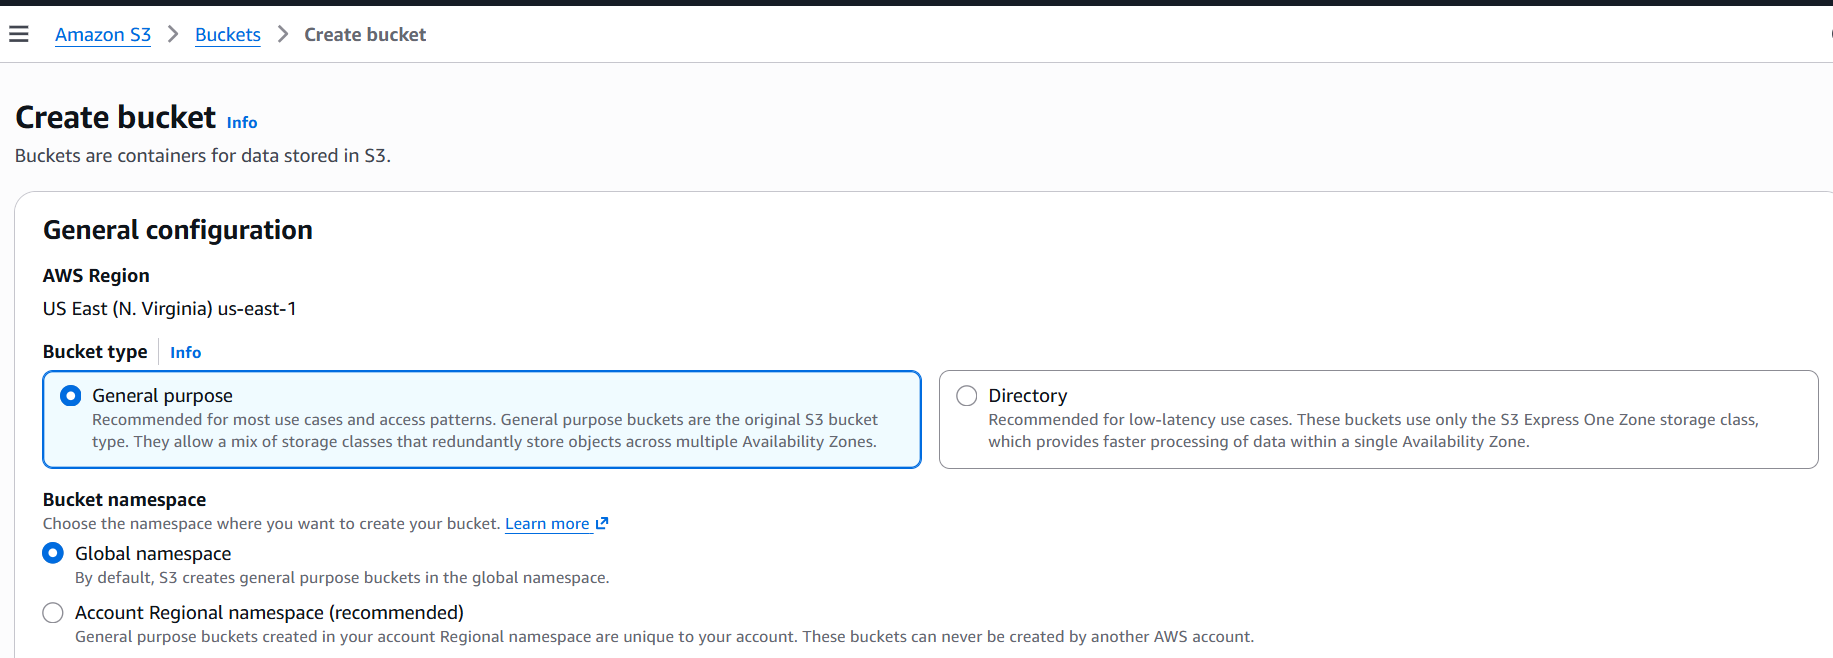
\includegraphics[width=10cm]{static/images/5-Workshop/5.4-S3-CloudFront/02-create-bucket.png}
        \caption{Trang ``Create bucket'' trên S3 Console}
        \label{fig:s3-create}
    \end{figure}

    \begin{figure}[H]
        \centering
        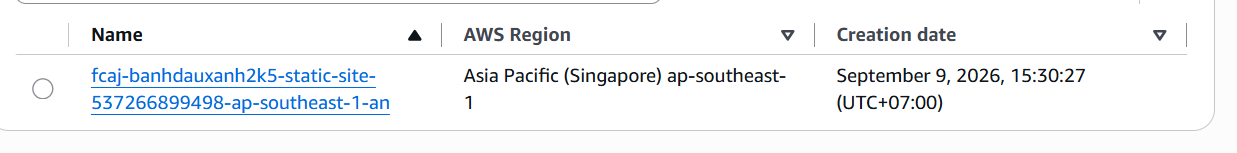
\includegraphics[width=10cm]{static/images/5-Workshop/5.4-S3-CloudFront/03-bucket-created.png}
        \caption{S3 Bucket đã được tạo và hiển thị trong danh sách}
        \label{fig:s3-created}
    \end{figure}

    \item Upload file \texttt{index.html} lên bucket. Vào tab
    \textit{Properties} → \textit{Static website hosting} → Enable, Index
    document: \texttt{index.html}.

    \begin{figure}[H]
        \centering
        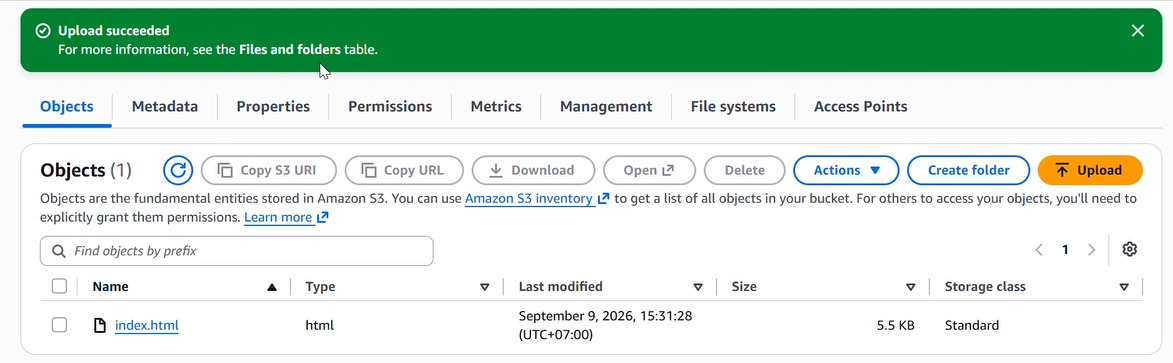
\includegraphics[width=10cm]{static/images/5-Workshop/5.4-S3-CloudFront/04-upload-files.png}
        \caption{Upload \texttt{index.html} lên S3 Bucket}
        \label{fig:s3-upload}
    \end{figure}

    \begin{figure}[H]
        \centering
        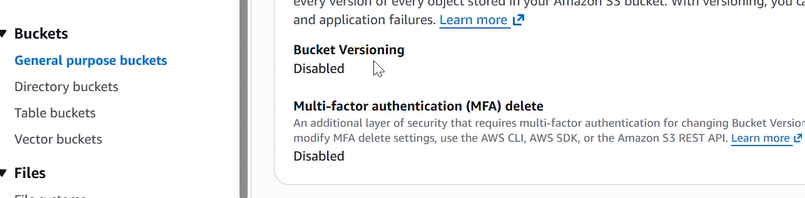
\includegraphics[width=10cm]{static/images/5-Workshop/5.4-S3-CloudFront/05-static-hosting-enable.png}
        \caption{Static website hosting: Enabled}
        \label{fig:s3-hosting}
    \end{figure}

    \item Vào tab \textit{Permissions} → \textit{Bucket policy}, thêm policy
    cho phép \texttt{s3:GetObject} công khai trên toàn bộ object trong
    bucket.

    \begin{figure}[H]
        \centering
        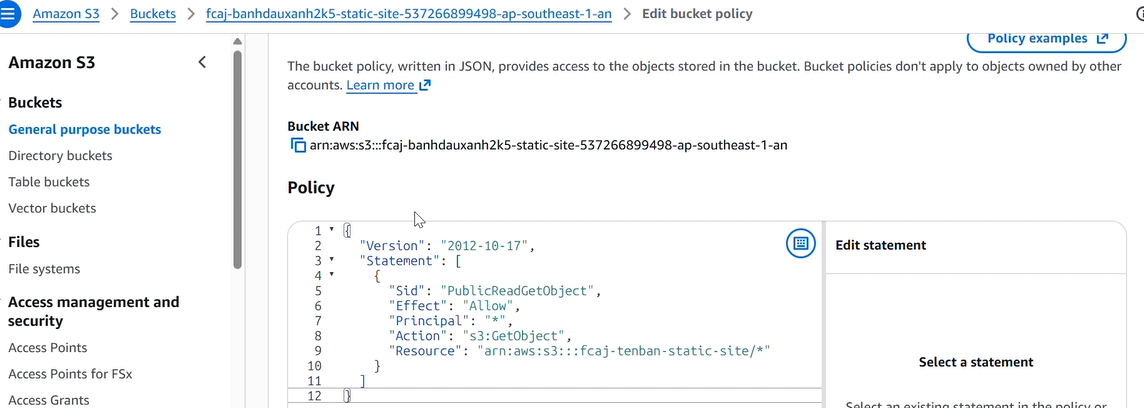
\includegraphics[width=10cm]{static/images/5-Workshop/5.4-S3-CloudFront/06-bucket-policy.png}
        \caption{Bucket policy cho phép \texttt{s3:GetObject} công khai}
        \label{fig:s3-policy}
    \end{figure}

    \item Tạo CloudFront Distribution, Origin domain trỏ về bucket vừa tạo,
    Viewer protocol policy: \textit{Redirect HTTP to HTTPS}.

    \begin{figure}[H]
        \centering
        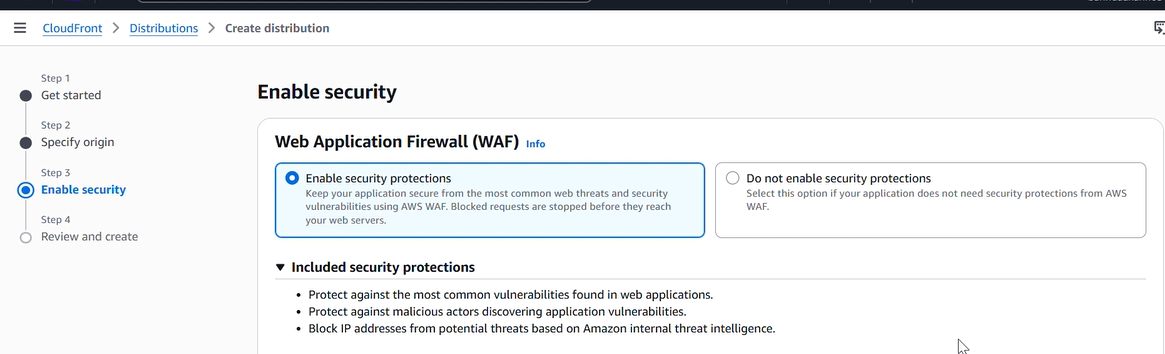
\includegraphics[width=10cm]{static/images/5-Workshop/5.4-S3-CloudFront/07-cloudfront-create.png}
        \caption{Trang tạo CloudFront Distribution}
        \label{fig:cf-create}
    \end{figure}

    \item Đợi Distribution chuyển sang trạng thái \textit{Enabled}.

    \begin{figure}[H]
        \centering
        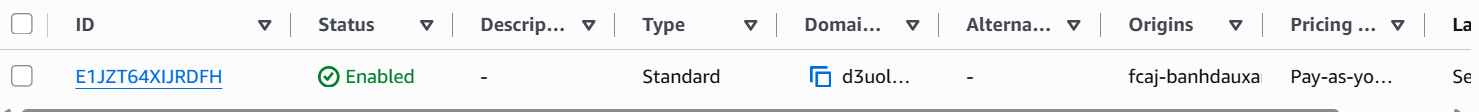
\includegraphics[width=10cm]{static/images/5-Workshop/5.4-S3-CloudFront/08-cloudfront-enabled.png}
        \caption{CloudFront Distribution ở trạng thái Enabled}
        \label{fig:cf-enabled}
    \end{figure}

    \item Mở Distribution domain name trên trình duyệt để kiểm thử -- website
    tải thành công qua HTTPS với ổ khóa bảo mật.

    \begin{figure}[H]
        \centering
        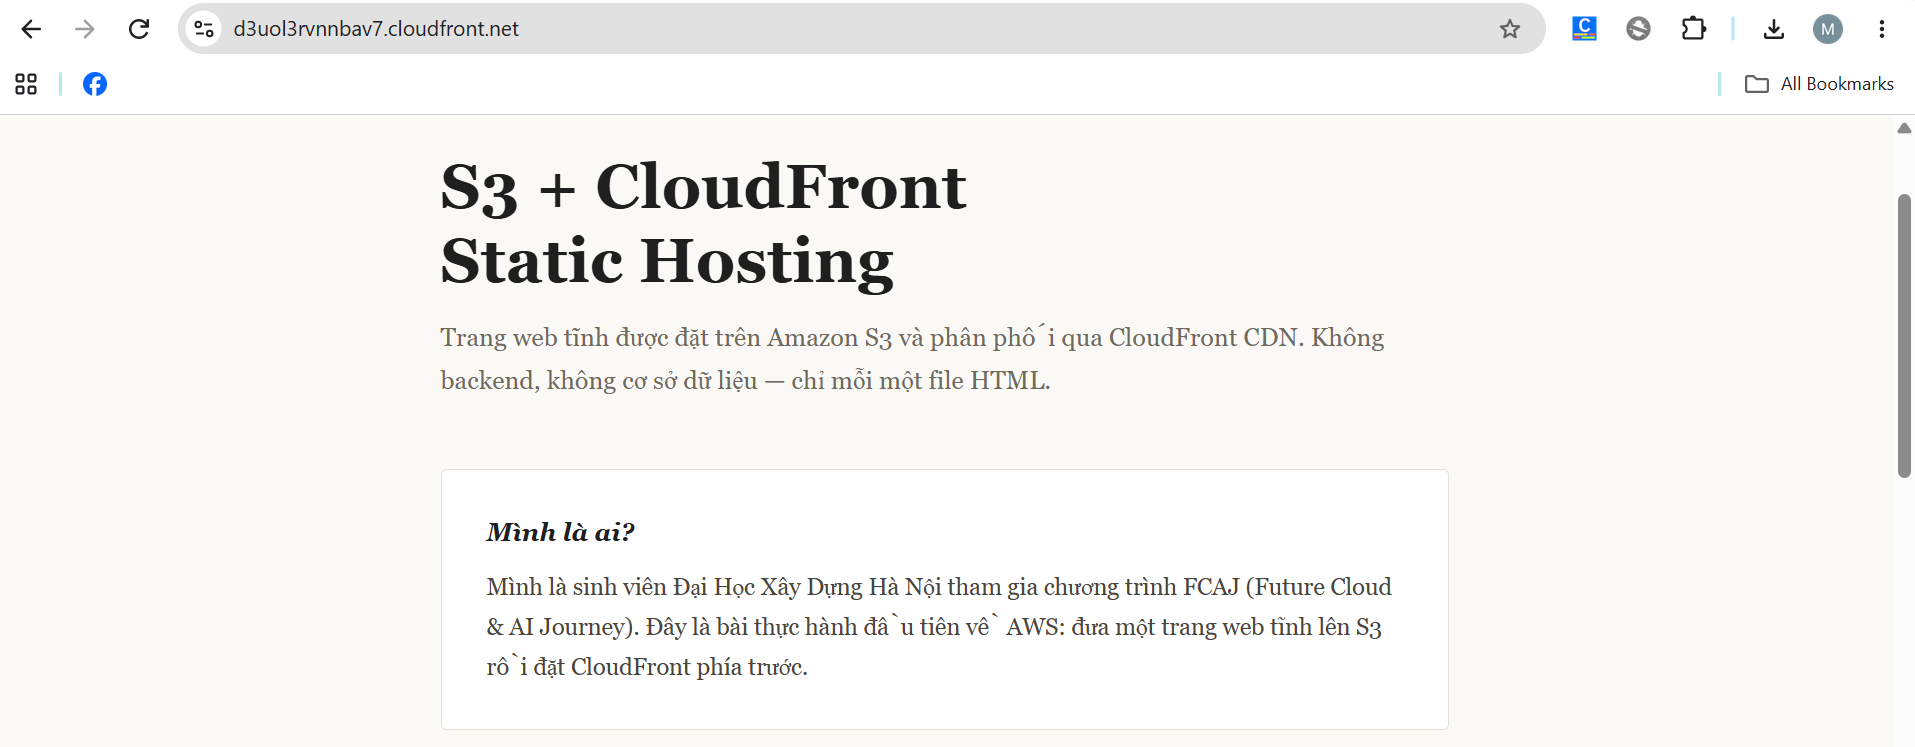
\includegraphics[width=10cm]{static/images/5-Workshop/5.4-S3-CloudFront/09-site-https.png}
        \caption{Trang web tải thành công qua CloudFront HTTPS}
        \label{fig:cf-site}
    \end{figure}
\end{enumerate}

\subsection{Xây dựng Serverless API (Lambda + API Gateway + DynamoDB)}

Workshop này xây dựng một API ghi chú (Notes API) hoàn toàn serverless: không cần
quản lý server, mọi thứ chạy trên nền tảng serverless của AWS.

Sơ đồ kiến trúc: Client $\rightarrow$ API Gateway (HTTP API) $\rightarrow$ Lambda
(Python 3.12) $\rightarrow$ DynamoDB (\texttt{fcaj-notes}).

\begin{enumerate}[leftmargin=1.5cm]
    \item Tạo bảng DynamoDB \texttt{fcaj-notes}, Partition key: \texttt{id}
    (String), giữ nguyên Default settings (on-demand).

    \begin{figure}[H]
        \centering
        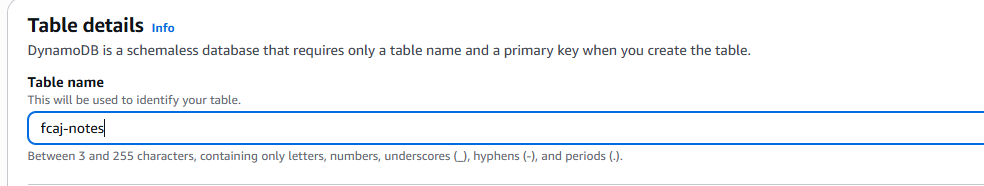
\includegraphics[width=10cm]{static/images/5-Workshop/5.5-Serverless-API/02-dynamodb-create-table.png}
        \caption{Trang ``Create table'' cho \texttt{fcaj-notes}}
        \label{fig:dynamo-create}
    \end{figure}

    \begin{figure}[H]
        \centering
        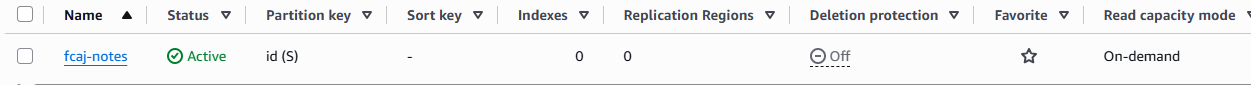
\includegraphics[width=10cm]{static/images/5-Workshop/5.5-Serverless-API/03-table-created.png}
        \caption{Bảng \texttt{fcaj-notes} đã được tạo}
        \label{fig:dynamo-created}
    \end{figure}

    \item Tạo IAM Role cho Lambda với 2 policy:
    \texttt{AWSLambdaBasicExecutionRole} và \texttt{AmazonDynamoDBFullAccess}.

    \begin{figure}[H]
        \centering
        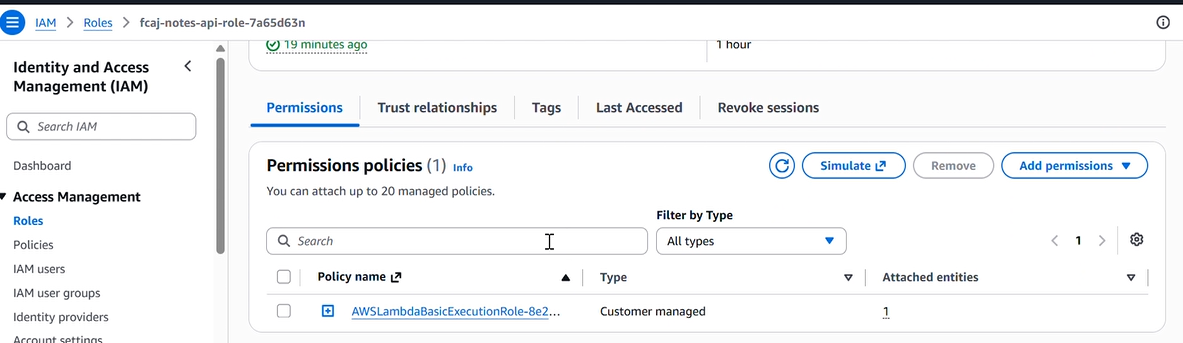
\includegraphics[width=10cm]{static/images/5-Workshop/5.5-Serverless-API/04-iam-role-lambda.png}
        \caption{IAM Role cho Lambda với 2 policy đã gắn}
        \label{fig:iam-lambda}
    \end{figure}

    \item Tạo Lambda function \texttt{fcaj-notes-api}, Runtime Python 3.12,
    gắn IAM Role vừa tạo. Viết mã xử lý 2 method \texttt{GET} (liệt kê
    note) và \texttt{POST} (thêm note mới), Deploy.

    \begin{figure}[H]
        \centering
        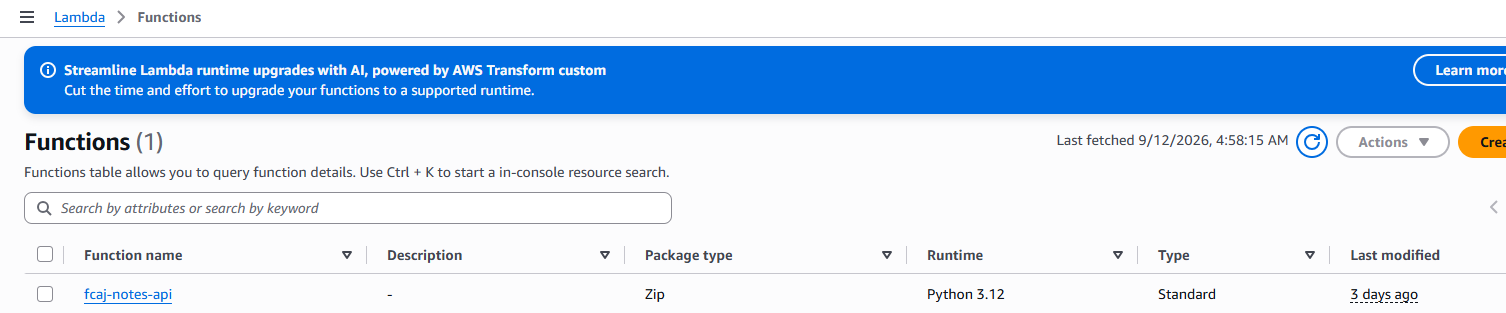
\includegraphics[width=10cm]{static/images/5-Workshop/5.5-Serverless-API/05-lambda-create.png}
        \caption{Trang tạo Lambda function}
        \label{fig:lambda-create}
    \end{figure}

    \begin{figure}[H]
        \centering
        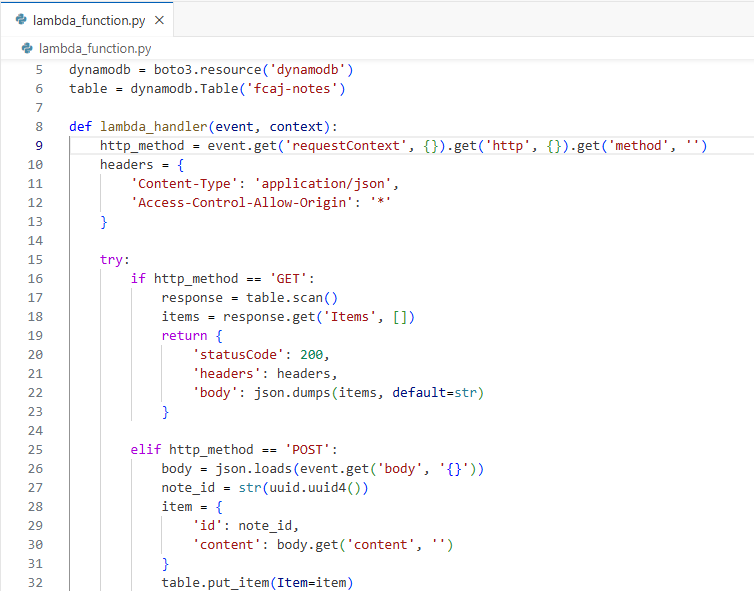
\includegraphics[width=10cm]{static/images/5-Workshop/5.5-Serverless-API/06-lambda-code.png}
        \caption{Mã nguồn Lambda function}
        \label{fig:lambda-code}
    \end{figure}

    \item Tạo HTTP API trên API Gateway, tích hợp với Lambda function, cấu
    hình 2 route: \texttt{GET /notes} và \texttt{POST /notes}.

    \begin{figure}[H]
        \centering
        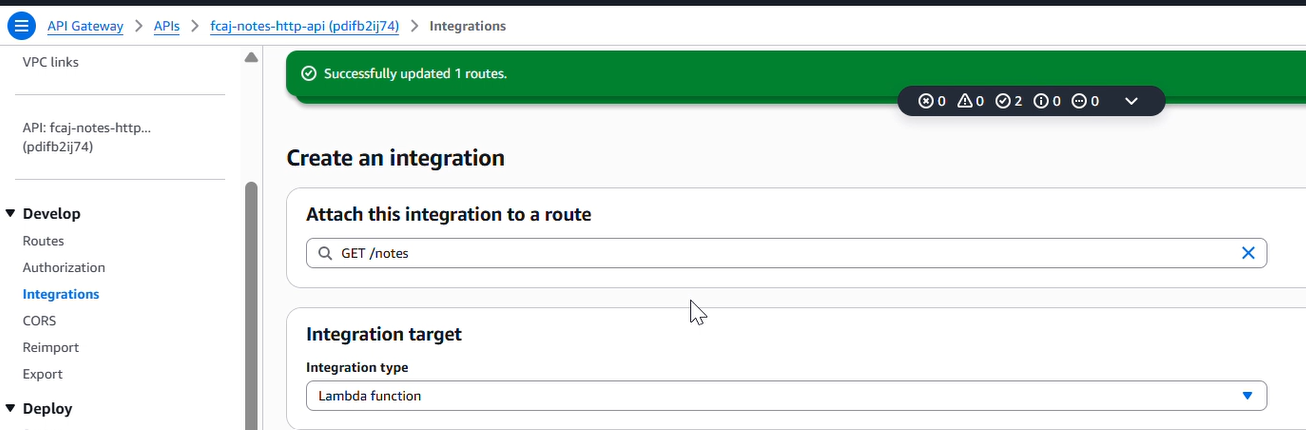
\includegraphics[width=10cm]{static/images/5-Workshop/5.5-Serverless-API/07-apigw-create.png}
        \caption{Đang tạo HTTP API và tích hợp với Lambda}
        \label{fig:apigw-create}
    \end{figure}

    \begin{figure}[H]
        \centering
        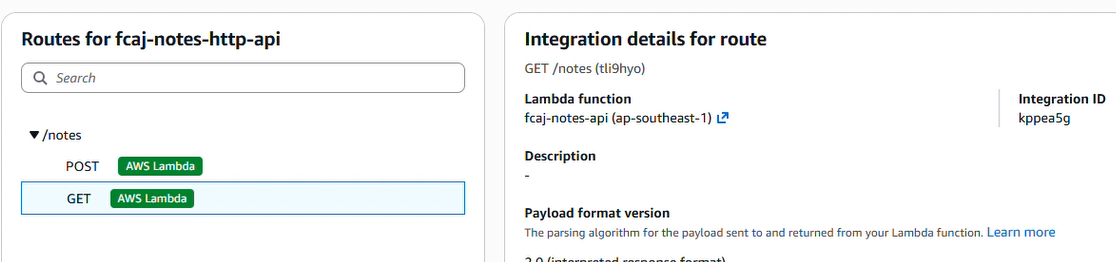
\includegraphics[width=10cm]{static/images/5-Workshop/5.5-Serverless-API/08-apigw-routes.png}
        \caption{Danh sách route trên API Gateway}
        \label{fig:apigw-routes}
    \end{figure}

    \item Kiểm thử: gọi \texttt{GET /notes} (trả về mảng rỗng ban đầu),
    sau đó \texttt{POST /notes} với nội dung mẫu, gọi lại \texttt{GET
    /notes} để xác nhận dữ liệu đã được lưu vào DynamoDB.

    \begin{figure}[H]
        \centering
        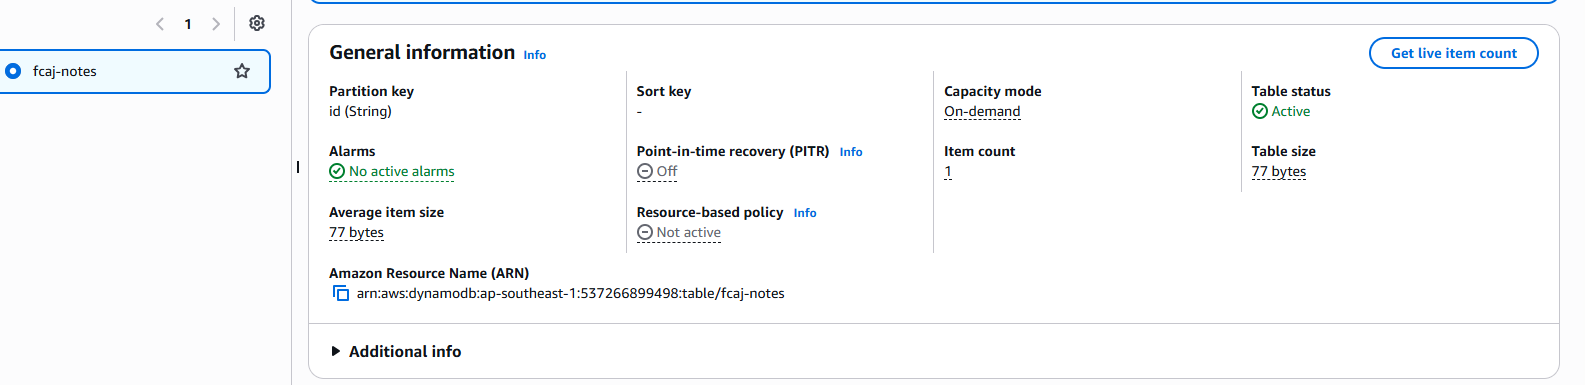
\includegraphics[width=10cm]{static/images/5-Workshop/5.5-Serverless-API/09-dynamodb-item.png}
        \caption{Bảng DynamoDB có item vừa thêm}
        \label{fig:dynamo-item}
    \end{figure}

    \begin{figure}[H]
        \centering
        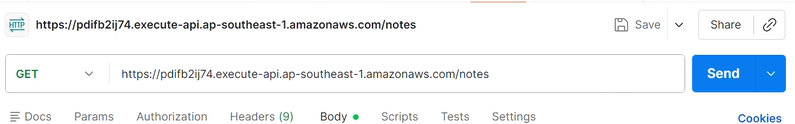
\includegraphics[width=10cm]{static/images/5-Workshop/5.5-Serverless-API/10-postman-get.png}
        \caption{Kết quả GET /notes thành công trên Postman}
        \label{fig:postman-get}
    \end{figure}

    \begin{figure}[H]
        \centering
        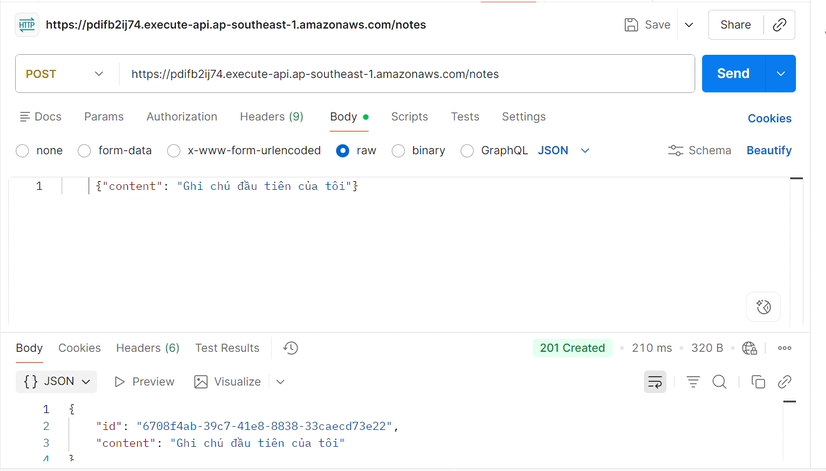
\includegraphics[width=10cm]{static/images/5-Workshop/5.5-Serverless-API/11-postman-post.png}
        \caption{Kết quả POST /notes thành công trên Postman}
        \label{fig:postman-post}
    \end{figure}
\end{enumerate}

\subsection{Thiết kế mạng VPC 2-tier}

Workshop này thiết kế mạng VPC 2 tầng -- mô hình được tái sử dụng cho dự án chính
Task Manager API: public subnet cho EC2 tiếp xúc internet và private subnet riêng
dành cho tầng database.

Sơ đồ kiến trúc: Internet $\rightarrow$ Internet Gateway $\rightarrow$ Public Subnet
(EC2) | Private Subnet -- cả hai nằm trong cùng VPC \texttt{10.0.0.0/16}.

\begin{enumerate}[leftmargin=1.5cm]
    \item Tạo VPC (CIDR \texttt{10.0.0.0/16}), sau đó tạo 2 subnet:
    Public subnet (\texttt{10.0.1.0/24}) và Private subnet
    (\texttt{10.0.2.0/24}), đặt ở 2 Availability Zone khác nhau.

    \begin{figure}[H]
        \centering
        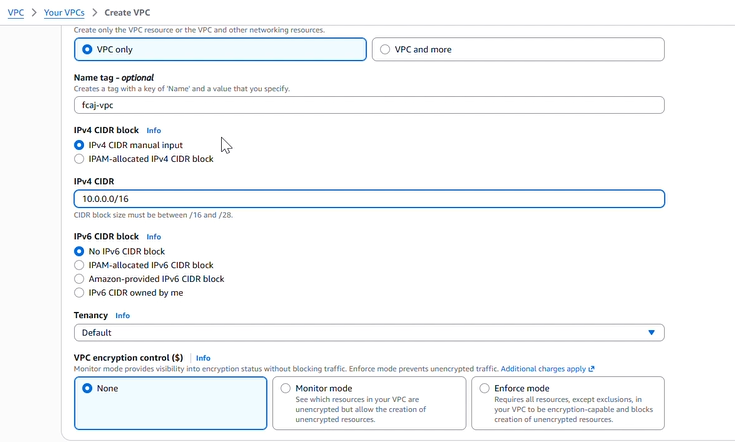
\includegraphics[width=10cm]{static/images/5-Workshop/5.6-VPC-2Tier/02-create-vpc.png}
        \caption{Đang tạo VPC với CIDR \texttt{10.0.0.0/16}}
        \label{fig:vpc-create}
    \end{figure}

    \begin{figure}[H]
        \centering
        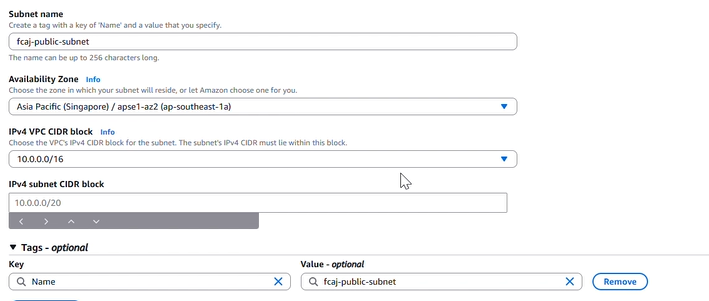
\includegraphics[width=10cm]{static/images/5-Workshop/5.6-VPC-2Tier/03-create-subnets.png}
        \caption{Hai subnet -- Public và Private}
        \label{fig:vpc-subnets}
    \end{figure}

    \item Tạo Internet Gateway, gắn vào VPC. Tạo Route Table cho Public
    subnet, thêm route \texttt{0.0.0.0/0} → Internet Gateway, gán vào
    Public subnet (Private subnet dùng Main route table mặc định, không có
    đường ra internet).

    \begin{figure}[H]
        \centering
        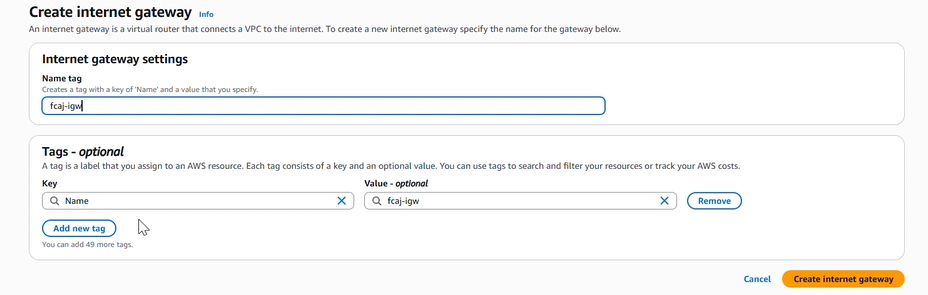
\includegraphics[width=10cm]{static/images/5-Workshop/5.6-VPC-2Tier/04-create-igw.png}
        \caption{Internet Gateway đã được gắn vào VPC}
        \label{fig:vpc-igw}
    \end{figure}

    \begin{figure}[H]
        \centering
        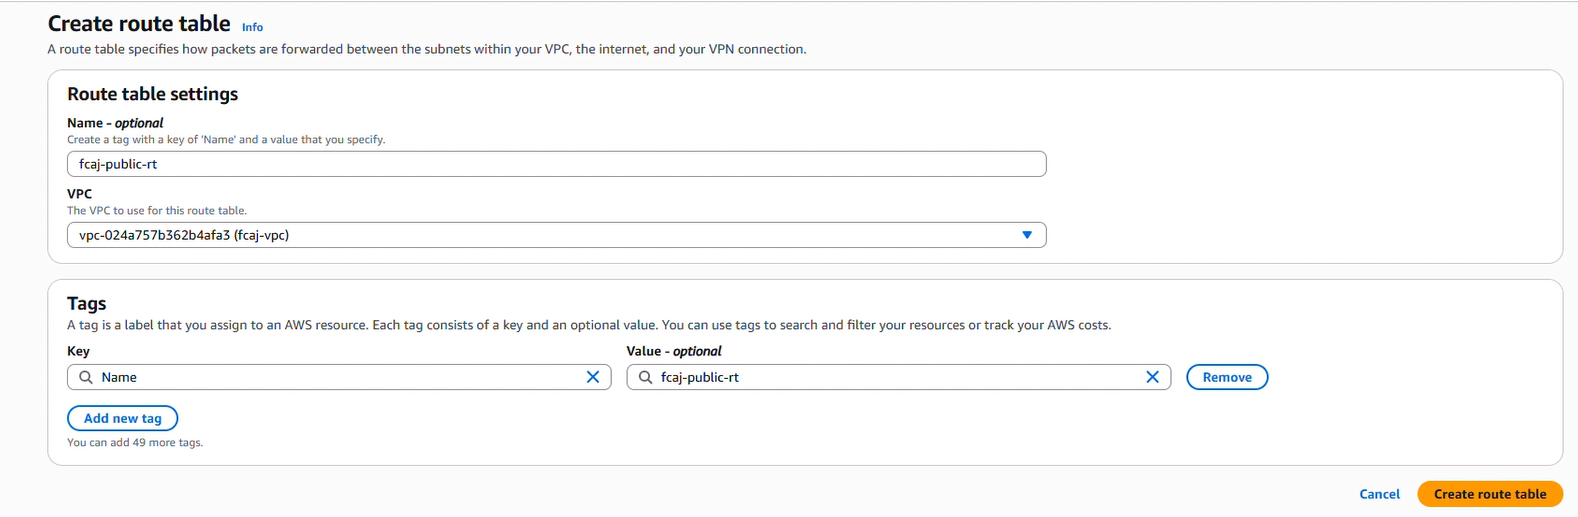
\includegraphics[width=10cm]{static/images/5-Workshop/5.6-VPC-2Tier/05-route-table.png}
        \caption{Route Table với \texttt{0.0.0.0/0} → Internet Gateway}
        \label{fig:vpc-route}
    \end{figure}

    \item Tạo Security Group cho phép SSH (port 22, nguồn: My IP) và HTTP
    (port 80, nguồn: Anywhere).

    \begin{figure}[H]
        \centering
        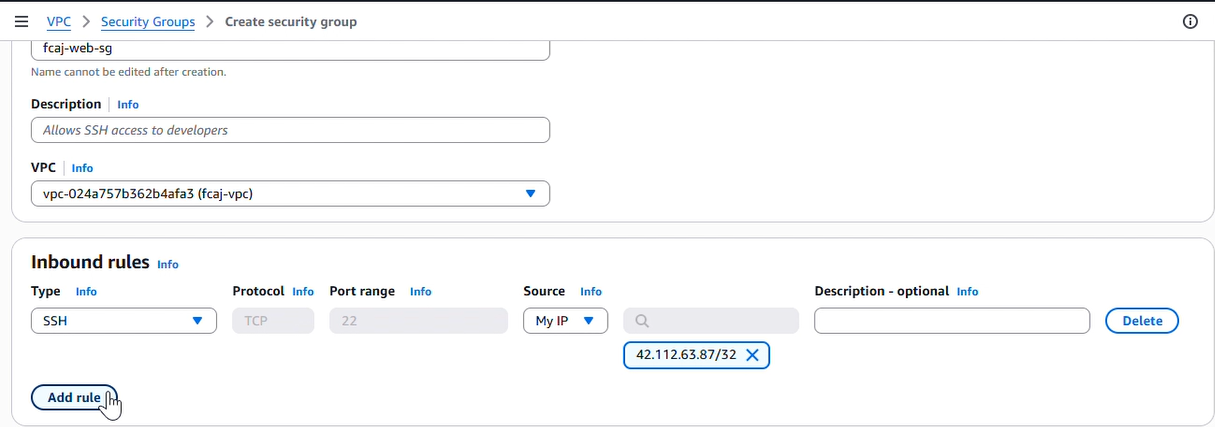
\includegraphics[width=10cm]{static/images/5-Workshop/5.6-VPC-2Tier/06-sg-create.png}
        \caption{Đang tạo Security Group}
        \label{fig:vpc-sg-create}
    \end{figure}

    \begin{figure}[H]
        \centering
        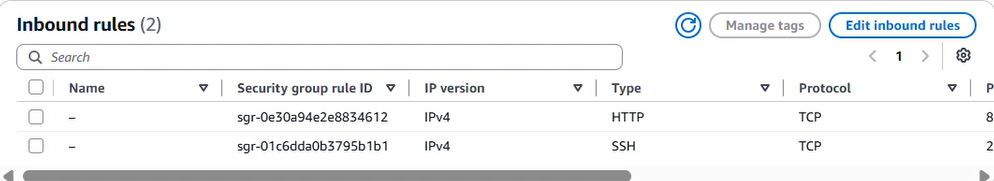
\includegraphics[width=10cm]{static/images/5-Workshop/5.6-VPC-2Tier/07-sg-rules.png}
        \caption{Inbound rules: SSH (22) và HTTP (80)}
        \label{fig:vpc-sg-rules}
    \end{figure}

    \item Khởi chạy EC2 instance (Amazon Linux 2023, t2.micro) trong Public
    subnet, bật Auto-assign public IP, gắn Security Group vừa tạo.

    \begin{figure}[H]
        \centering
        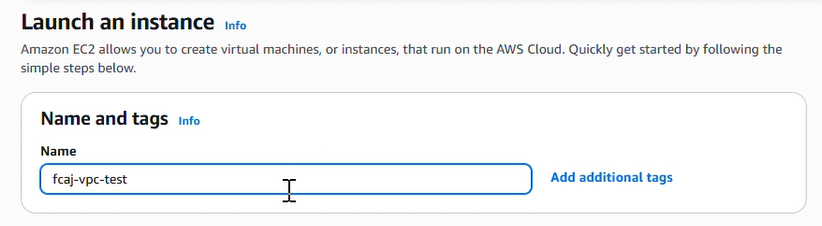
\includegraphics[width=10cm]{static/images/5-Workshop/5.6-VPC-2Tier/08-launch-ec2.png}
        \caption{Đang khởi chạy EC2 instance Amazon Linux 2023 t2.micro}
        \label{fig:vpc-ec2-launch}
    \end{figure}

    \begin{figure}[H]
        \centering
        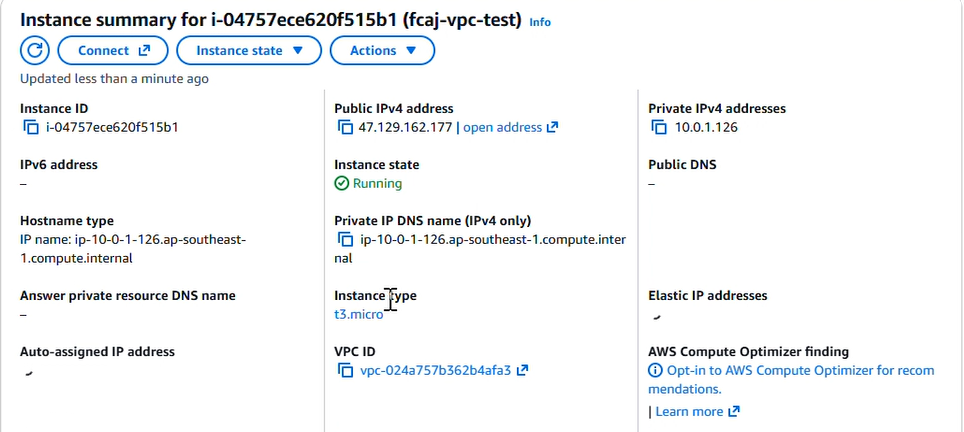
\includegraphics[width=10cm]{static/images/5-Workshop/5.6-VPC-2Tier/09-ec2-running.png}
        \caption{EC2 instance ở trạng thái Running}
        \label{fig:vpc-ec2-running}
    \end{figure}

    \item Kiểm thử kết nối SSH từ máy cá nhân tới EC2 bằng key pair -- kết
    nối thành công.

    \begin{figure}[H]
        \centering
        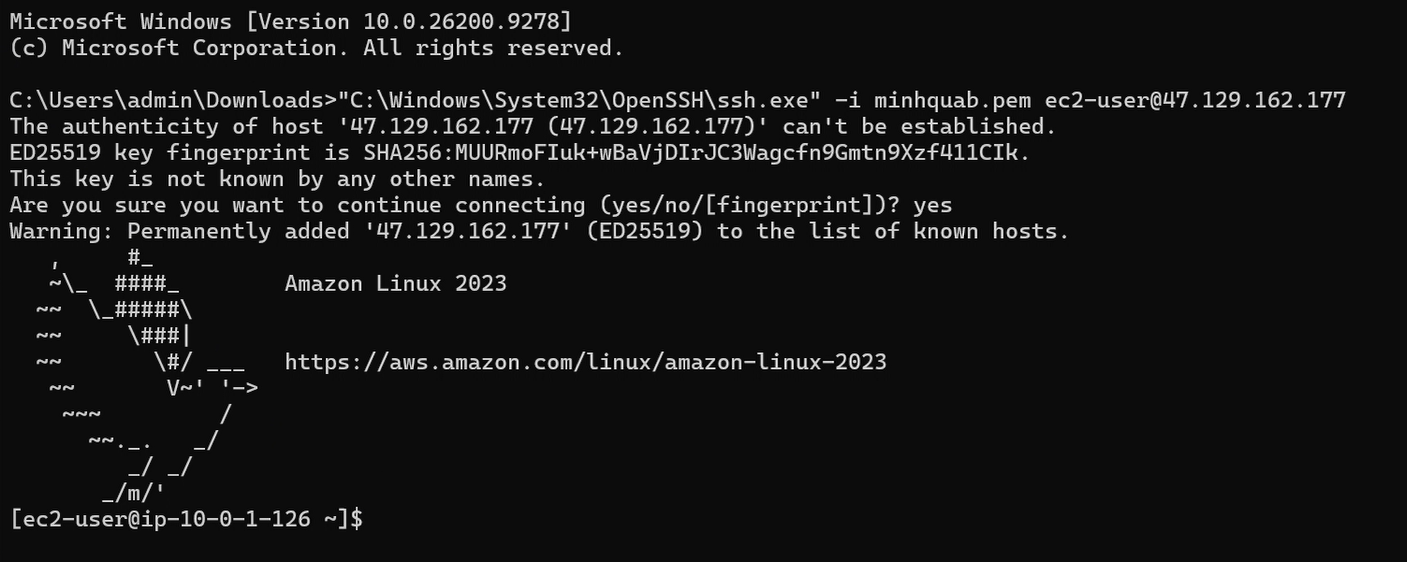
\includegraphics[width=10cm]{static/images/5-Workshop/5.6-VPC-2Tier/10-ssh-success.png}
        \caption{Kết nối SSH thành công tới EC2 instance}
        \label{fig:vpc-ssh}
    \end{figure}
\end{enumerate}

\subsection{Dự án chính: Task Manager API (EC2 + RDS + AI)}

Dự án Task Manager API là nội dung thực hành trọng tâm của đợt thực tập,
thay thế cho một workshop EC2 đơn giản trong kế hoạch ban đầu bằng một hệ
 thống hoàn chỉnh: Backend Java Spring Boot triển khai trên EC2, cơ sở dữ
liệu MySQL trên RDS, Frontend HTML/CSS/JS trên Nginx, và tích hợp AI (Amazon
Comprehend) để đáp ứng CLO3 của học phần.

\subsubsection{Mô tả bài toán và kiến trúc hệ thống}

Task Manager API là REST API Backend phục vụ quản lý công việc/dự án ở quy
mô nhỏ: người dùng đăng ký/đăng nhập, tạo và quản lý các dự án (Project),
tạo/quản lý các công việc (Task) thuộc từng dự án với trạng thái TODO,
IN\_PROGRESS, DONE. Mỗi task khi tạo/cập nhật sẽ được AI (Amazon Comprehend)
tự động phân tích để gợi ý mức độ ưu tiên.

Kiến trúc tổng thể tuân theo mô hình 3 tầng trong một VPC, được chia thành
bốn thành phần chính. Tầng \textbf{Frontend} gồm HTML/CSS/JavaScript thuần
do Nginx phục vụ trên EC2 (cổng 80). Tầng \textbf{Backend} là REST API Java
Spring Boot 3.3 chạy trên EC2 (cổng 8080, public subnet). Tầng
\textbf{Database} sử dụng MySQL 8.0 trên Amazon RDS (private subnet), chỉ
nhận kết nối từ Security Group của EC2 qua port 3306. Cuối cùng, thành phần
\textbf{AI Service} là Amazon Comprehend, được EC2 gọi qua IAM Role (không
hardcode Access Key) để phân tích sentiment và trích xuất từ khóa từ mô tả
task.

\begin{figure}[H]
    \centering
    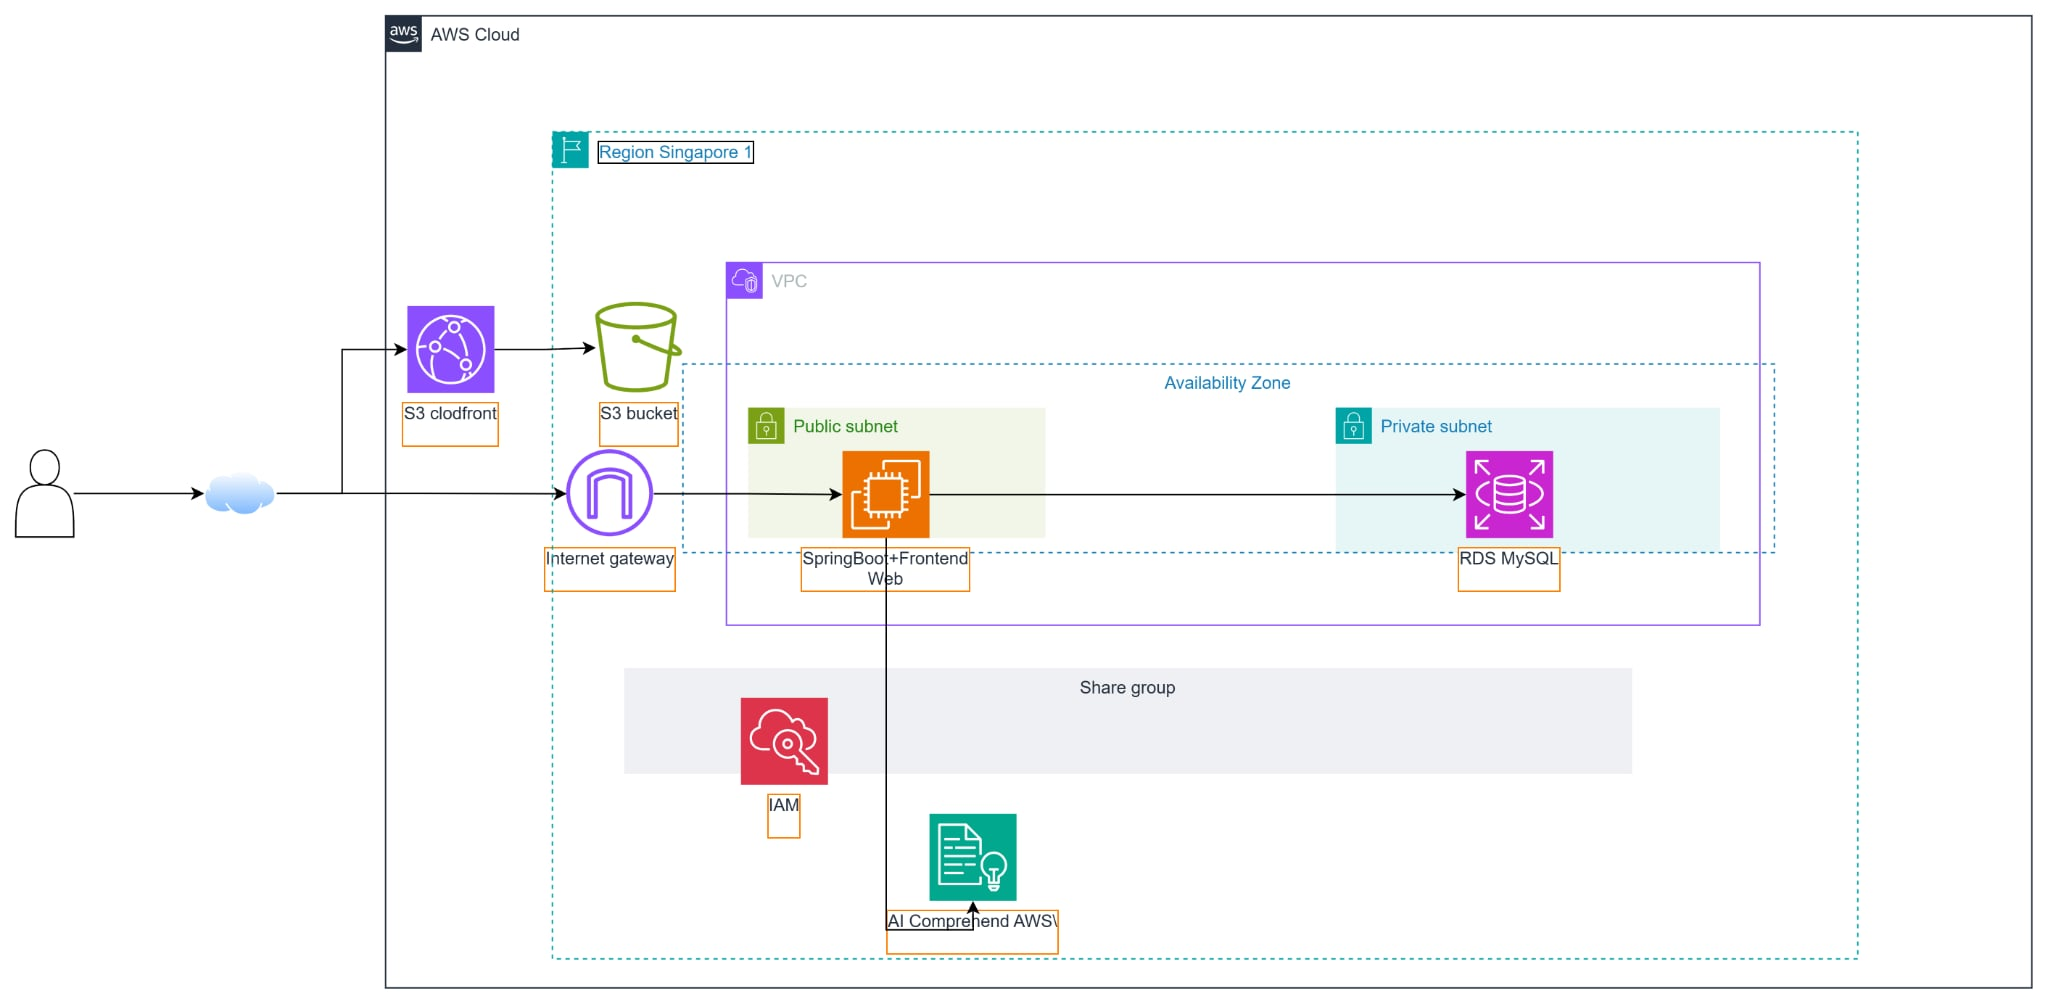
\includegraphics[width=12cm]{architecture.jpg}
    \caption{Kiến trúc tổng thể dự án Task Manager API}
    \label{fig:project-arch}
\end{figure}

\subsubsection{Công nghệ sử dụng}

\begin{longtable}{p{4cm}p{9.5cm}}
\caption{Danh mục công nghệ sử dụng trong dự án}
\label{tab:tech-stack} \\
\toprule
\textbf{Thành phần} & \textbf{Công nghệ} \\
\midrule
\endhead
Ngôn ngữ lập trình & Java 17 \\
Framework Backend & Spring Boot 3.3, Spring Security, Spring Data JPA \\
Xác thực & JWT (JSON Web Token), mã hóa mật khẩu BCrypt \\
Cơ sở dữ liệu & MySQL 8.x (Amazon RDS, \texttt{db.t3.micro}) \\
Dịch vụ AI & Amazon Comprehend (DetectSentiment, DetectKeyPhrases) \\
Frontend & HTML5, CSS3, JavaScript thuần (Fetch API), Nginx (web server) \\
Đóng gói \& triển khai & Apache Maven, Docker, Docker Compose \\
Hạ tầng Cloud & Amazon EC2 (\texttt{t3.micro}), Amazon RDS, Amazon VPC 2-tier, IAM Role \\
Công cụ build & Apache Maven (\texttt{mvn clean package -DskipTests}) \\
Công cụ kiểm thử API & Postman, curl \\
\bottomrule
\end{longtable}

\subsubsection{Thiết kế cơ sở dữ liệu}

Hệ thống sử dụng 3 bảng dữ liệu chính: \texttt{users}, \texttt{projects},
\texttt{tasks}. Bảng \texttt{tasks} có bổ sung 2 cột phục vụ tính năng AI:
\texttt{priority} (LOW/MEDIUM/HIGH, do AI gợi ý) và \texttt{ai\_key\_phrases}
(các từ khóa do Comprehend trích xuất). Quan hệ: một user sở hữu nhiều
project (1--N), một project chứa nhiều task (1--N), một task có thể được
gán cho một user (assignee, quan hệ N--1).

\begin{longtable}{p{3cm}p{4cm}p{6cm}}
\caption{Cấu trúc 3 bảng dữ liệu chính}
\label{tab:db-schema} \\
\toprule
\textbf{Bảng} & \textbf{Cột chính} & \textbf{Ghi chú} \\
\midrule
\endhead
users & id (PK), username, password, created\_at & Mã hóa mật khẩu bằng BCrypt \\
projects & id (PK), name, description, owner\_id (FK→users) & Quan hệ 1--N với users \\
tasks & id (PK), title, description, status, priority, ai\_key\_phrases, project\_id (FK→projects), assignee\_id (FK→users) & Status: TODO/IN\_PROGRESS/DONE; priority và ai\_key\_phrases do AI điền tự động \\
\bottomrule
\end{longtable}

\begin{figure}[H]
    \centering
    \fbox{\parbox{10cm}{\centering\vspace{2.5cm}[Sơ đồ ERD 3 bảng: users, projects,
    tasks -- vẽ bằng draw.io. File nguồn: \texttt{drawio/5.7-taskmanager-erd.drawio}]\vspace{2.5cm}}}
    \caption{Sơ đồ quan hệ thực thể (ERD) của Task Manager API}
    \label{fig:erd}
\end{figure}

\subsubsection{Thiết lập RDS MySQL}

\begin{enumerate}[leftmargin=1.5cm]
    \item Console → RDS → \textbf{Create database} → Engine: MySQL,
    Template: Free tier.

    \begin{figure}[H]
        \centering
        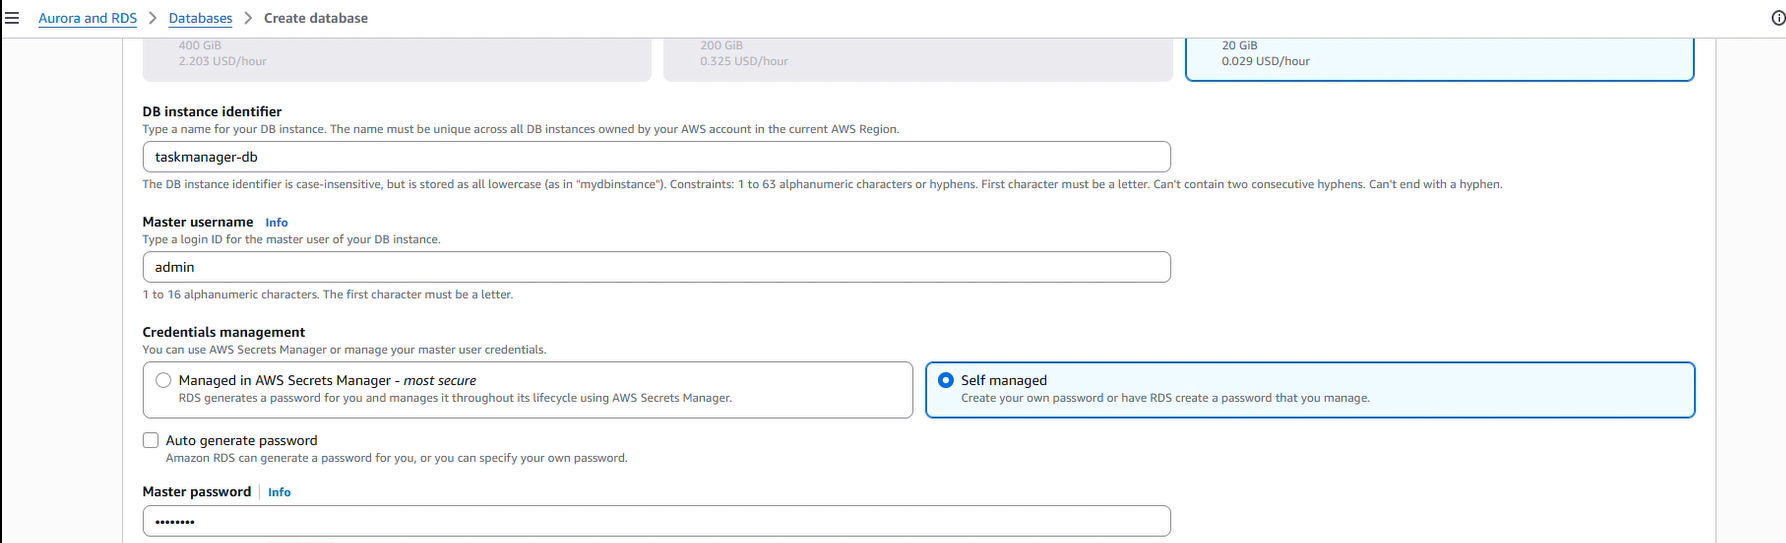
\includegraphics[width=10cm]{static/images/5-Workshop/5.8-TaskManager-RDS/01-rds-create.png}
        \caption{Trang ``Create database'' -- MySQL, Free tier}
        \label{fig:rds-create}
    \end{figure}

    \item DB instance identifier: \texttt{taskmanager-db}. Master username:
    \texttt{admin}, đặt password mạnh (lưu lại cẩn thận, không thể xem lại).
    DB instance class: \texttt{db.t3.micro}. Public access: \textbf{No}
    (giữ RDS ở chế độ private).

    \begin{figure}[H]
        \centering
        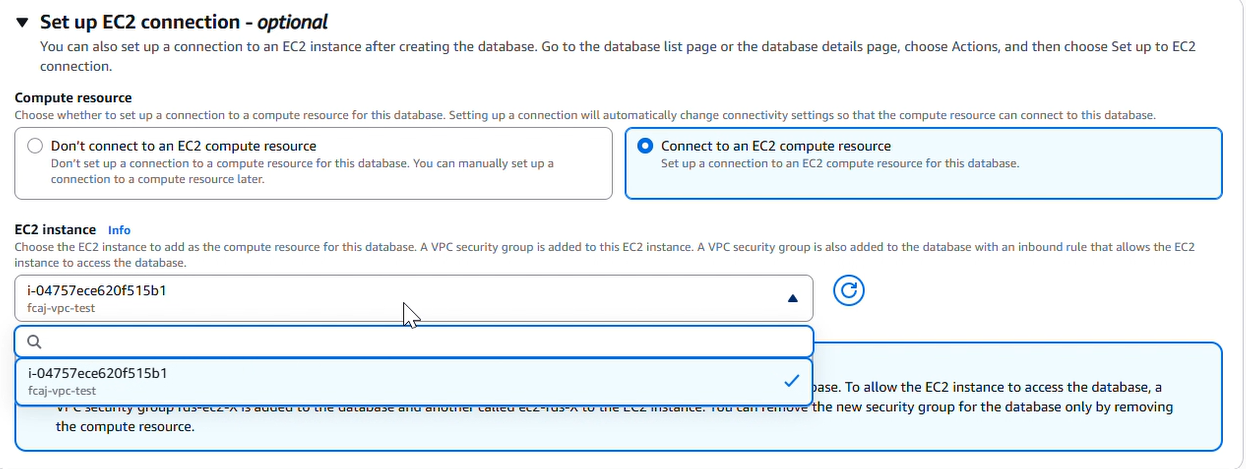
\includegraphics[width=10cm]{static/images/5-Workshop/5.8-TaskManager-RDS/02-rds-config.png}
        \caption{Cấu hình RDS -- private, không public access}
        \label{fig:rds-config}
    \end{figure}

    \item VPC security group: Create new, đặt tên \texttt{rds-sg}. Initial
    database name: \texttt{taskmanager}. \textbf{Create database}, đợi tới
    khi status chuyển \textit{Available}. Vào tab \textit{Connectivity \&
    security}, copy lại \textbf{Endpoint}.

    \begin{figure}[H]
        \centering
        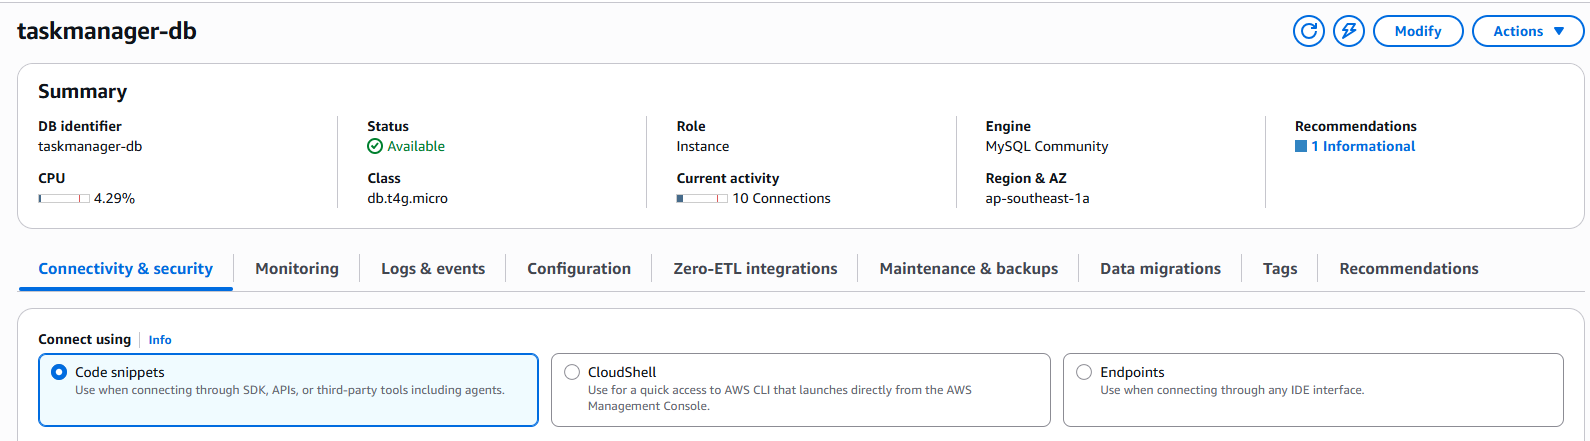
\includegraphics[width=10cm]{static/images/5-Workshop/5.8-TaskManager-RDS/03-rds-available.png}
        \caption{RDS instance ở trạng thái Available với Endpoint đầy đủ}
        \label{fig:rds-available}
    \end{figure}
\end{enumerate}

\subsubsection{Thiết lập EC2 và triển khai Backend}

\begin{enumerate}[leftmargin=1.5cm]
    \item Launch EC2 instance (Amazon Linux 2023, \texttt{t3.micro}) trong cùng VPC
    với RDS, Public subnet, Security Group mở port 22 (My IP) và 8080
    (Anywhere).

    \begin{figure}[H]
        \centering
        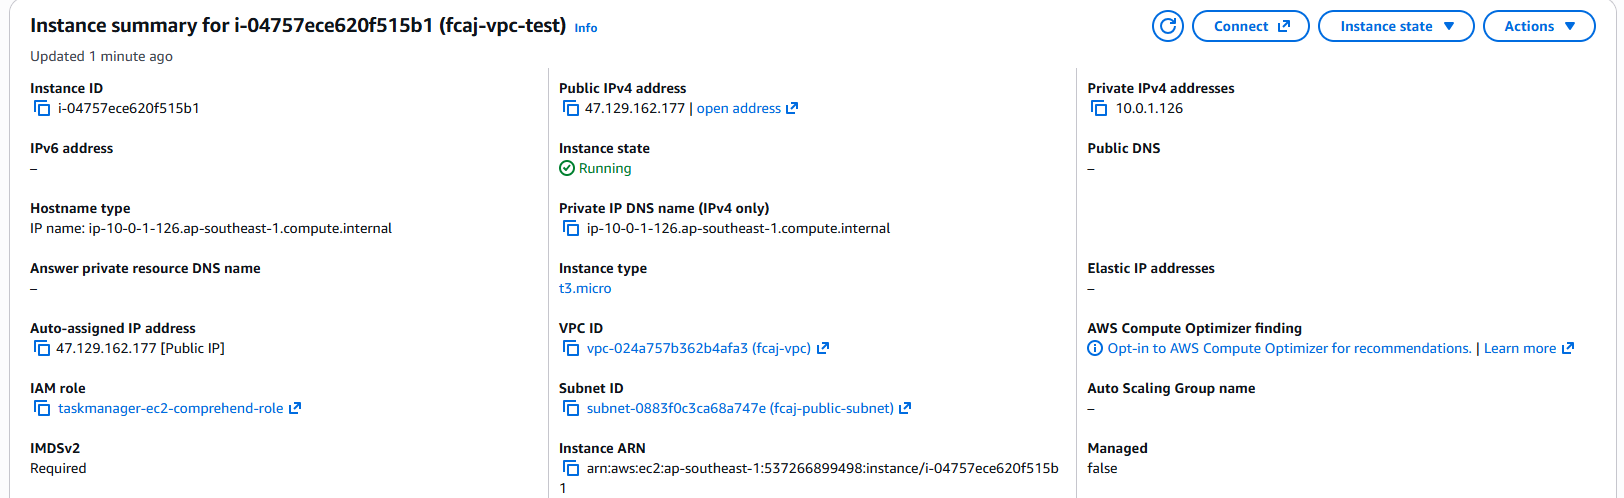
\includegraphics[width=10cm]{static/images/5-Workshop/5.9-TaskManager-EC2/01-ec2-launch.png}
        \caption{Đang khởi chạy EC2 instance Amazon Linux 2023 t3.micro}
        \label{fig:ec2-launch}
    \end{figure}

    \begin{figure}[H]
        \centering
        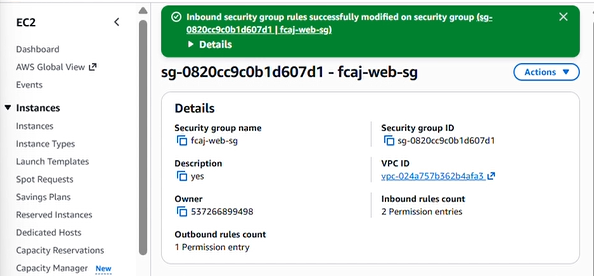
\includegraphics[width=10cm]{static/images/5-Workshop/5.9-TaskManager-EC2/02-ec2-running.png}
        \caption{EC2 instance backend ở trạng thái Running}
        \label{fig:ec2-running}
    \end{figure}

    \item Vào Security Group của RDS (\texttt{rds-sg}) → Edit inbound rules
    → thêm rule MYSQL/Aurora (port 3306), Source: Security Group của EC2
    (không mở Anywhere -- đây là best practice bảo mật).

    \begin{figure}[H]
        \centering
        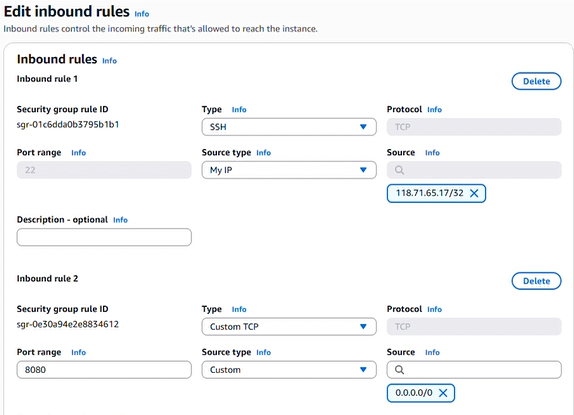
\includegraphics[width=10cm]{static/images/5-Workshop/5.9-TaskManager-EC2/03-rds-sg-inbound.png}
        \caption{Thêm inbound rule MySQL cho \texttt{rds-sg} -- source là Security Group của EC2}
        \label{fig:rds-sg-inbound}
    \end{figure}

    \item SSH vào EC2, cài Java 17: \texttt{sudo dnf install -y
    java-17-amazon-corretto-devel}.

    \begin{figure}[H]
        \centering
        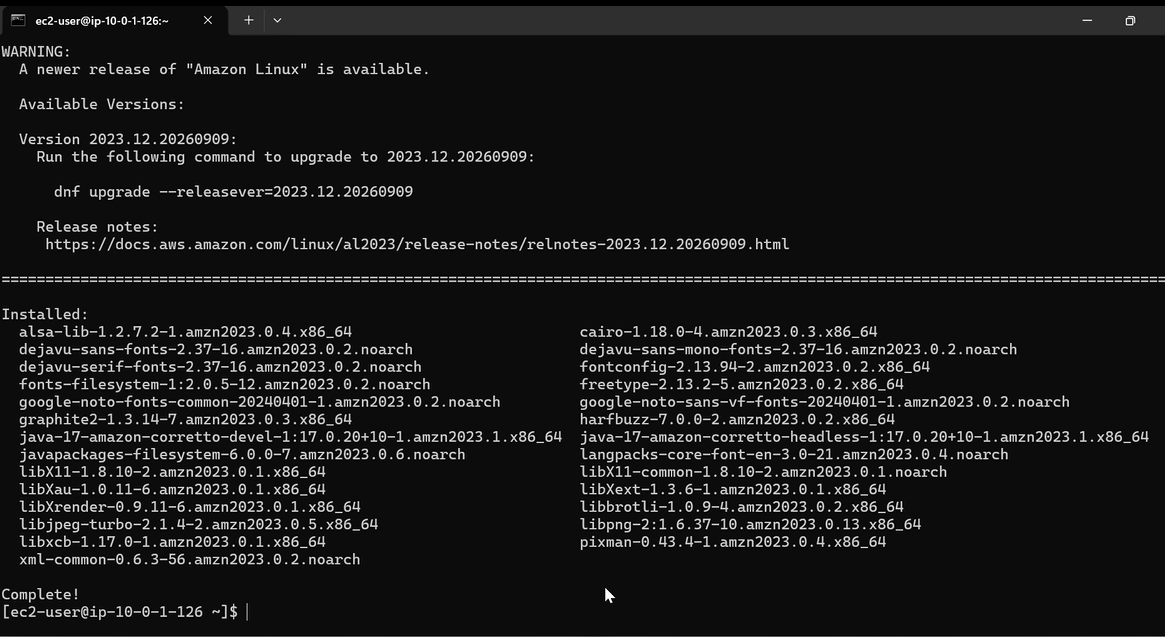
\includegraphics[width=10cm]{static/images/5-Workshop/5.9-TaskManager-EC2/04-install-java.png}
        \caption{Java 17 đã được cài trên EC2 instance}
        \label{fig:ec2-java}
    \end{figure}

    \item Build project trên máy local (\texttt{mvn clean package
    -DskipTests}), copy file \texttt{.jar} lên EC2 bằng \texttt{scp}.

    \item Tạo file \texttt{app.env} chứa các biến môi trường
    (\texttt{DB\_HOST}, \texttt{DB\_PORT}, \texttt{DB\_NAME},
    \texttt{DB\_USERNAME}, \texttt{DB\_PASSWORD}, \texttt{JWT\_SECRET}
    -- tối thiểu 32 ký tự, \texttt{AWS\_REGION}, \texttt{AI\_ENABLED}).
    Tạo systemd service để ứng dụng tự khởi động lại khi EC2 reboot.

    \item Khởi động service, kiểm tra log bằng
    \texttt{journalctl -u taskmanager -f} -- xác nhận dòng ``Started
    TaskManagerApiApplication''.

    \begin{figure}[H]
        \centering
        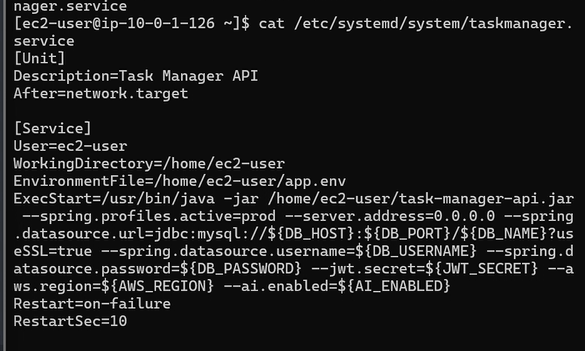
\includegraphics[width=10cm]{static/images/5-Workshop/5.9-TaskManager-EC2/05-backend-log.png}
        \caption{Log service hiển thị ``Started TaskManagerApiApplication''}
        \label{fig:ec2-log}
    \end{figure}

    \item Kiểm thử: gọi \texttt{POST /api/auth/register} -- trả về JWT
    token, xác nhận backend kết nối RDS thành công.

    \begin{figure}[H]
        \centering
        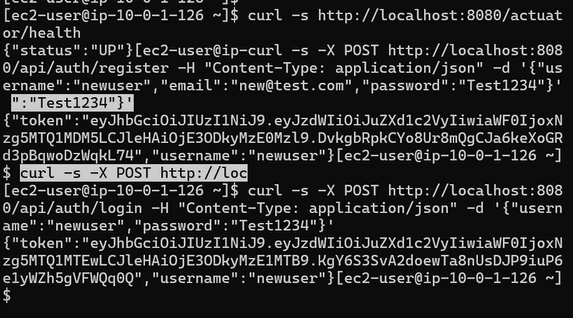
\includegraphics[width=10cm]{static/images/5-Workshop/5.9-TaskManager-EC2/06-register-jwt.png}
        \caption{Kết quả gọi \texttt{POST /api/auth/register} trả về JWT token}
        \label{fig:ec2-jwt}
    \end{figure}
\end{enumerate}

\subsubsection{Tích hợp AI: Amazon Comprehend qua IAM Role}

Đây là phần triển khai đáp ứng CLO3 (vận dụng kiến thức AI vào bài toán
thực tế). Thay vì hardcode Access Key/Secret Key -- vốn không an toàn --
hệ thống được cấp quyền gọi Comprehend thông qua \textbf{IAM Role} gắn trực
tiếp vào EC2 instance, theo đúng thực hành chuẩn (best practice) của AWS.

\begin{enumerate}[leftmargin=1.5cm]
    \item Console → IAM → \textbf{Roles} → \textbf{Create role}. Trusted
    entity: AWS service → Use case: \textbf{EC2}.

    \begin{figure}[H]
        \centering
        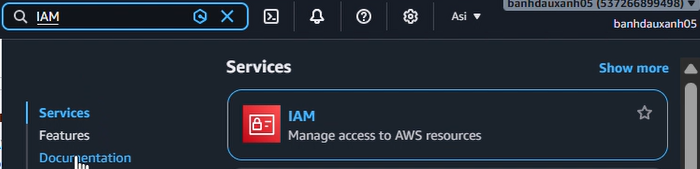
\includegraphics[width=10cm]{static/images/5-Workshop/5.10-TaskManager-AI/01-iam-create-role.png}
        \caption{Trang ``Create role'' trên IAM Console}
        \label{fig:iam-create}
    \end{figure}

    \item Ở bước Permissions, tìm và tick policy \textbf{ComprehendReadOnly}.

    \begin{figure}[H]
        \centering
        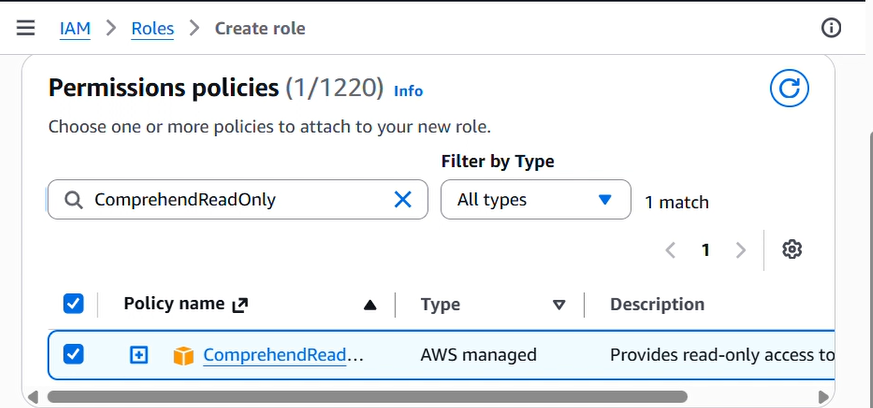
\includegraphics[width=10cm]{static/images/5-Workshop/5.10-TaskManager-AI/02-iam-comprehend-policy.png}
        \caption{Chọn policy \texttt{ComprehendReadOnly}}
        \label{fig:iam-policy}
    \end{figure}

    \item Đặt tên role: \texttt{taskmanager-ec2-comprehend-role} →
    \textbf{Create role}.

    \begin{figure}[H]
        \centering
        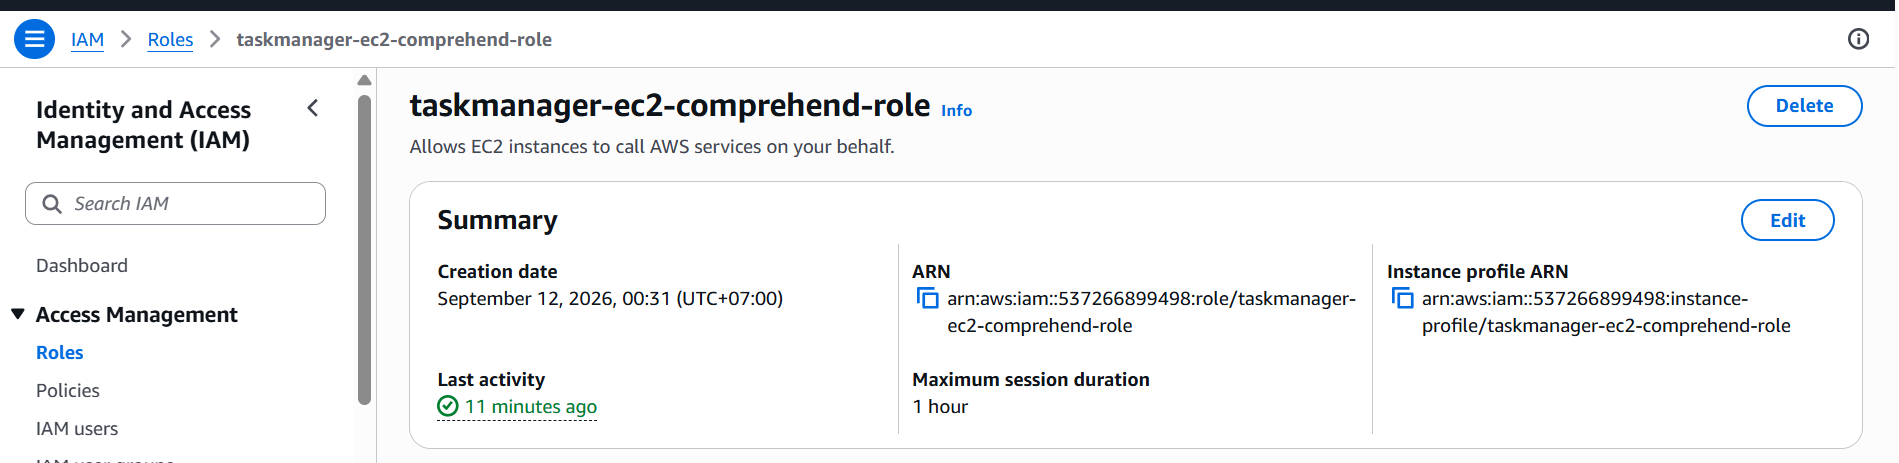
\includegraphics[width=10cm]{static/images/5-Workshop/5.10-TaskManager-AI/03-iam-role-created.png}
        \caption{IAM Role với policy \texttt{ComprehendReadOnly} đã tạo}
        \label{fig:iam-created}
    \end{figure}

    \item Quay lại EC2 Console → chọn instance đang chạy backend →
    \textbf{Actions → Security → Modify IAM role} → chọn role vừa tạo →
    \textbf{Update IAM role}.

    \begin{figure}[H]
        \centering
        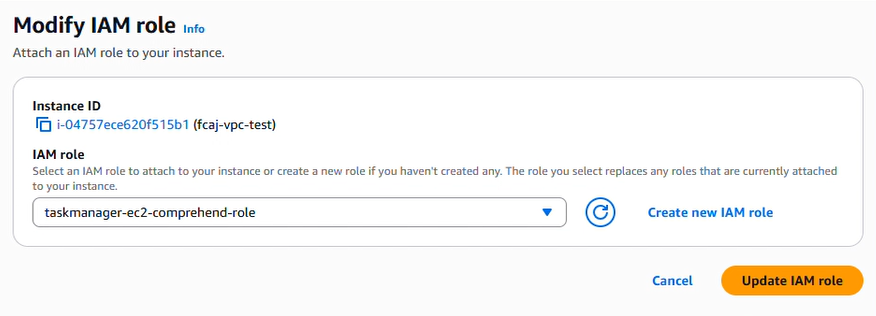
\includegraphics[width=10cm]{static/images/5-Workshop/5.10-TaskManager-AI/04-ec2-modify-iam-role.png}
        \caption{Chọn \texttt{taskmanager-ec2-comprehend-role} trong ``Modify IAM role''}
        \label{fig:ec2-modify-iam}
    \end{figure}

    \begin{figure}[H]
        \centering
        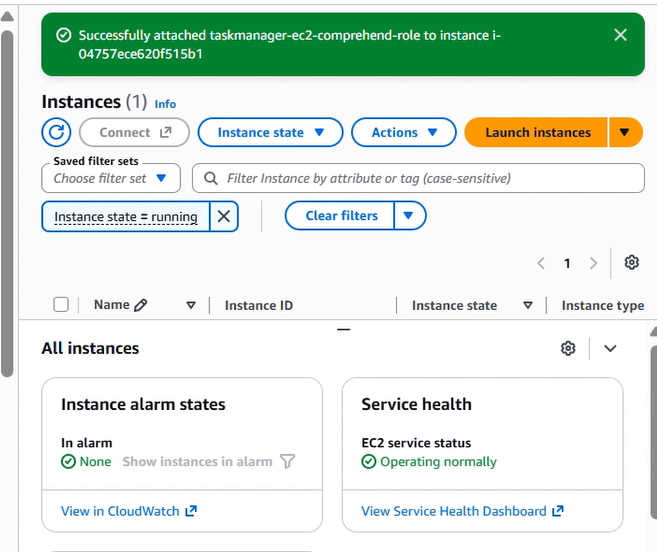
\includegraphics[width=10cm]{static/images/5-Workshop/5.10-TaskManager-AI/05-ec2-iam-role.png}
        \caption{EC2 instance details hiển thị IAM Role vừa gán}
        \label{fig:ec2-iam-role}
    \end{figure}

    \item Khởi động lại service backend (\texttt{sudo systemctl restart
    taskmanager}) để AWS SDK nhận quyền mới từ IAM Role.

    \item Kiểm thử: gọi API tạo task với nội dung mô tả có sắc thái khẩn
    cấp (ví dụ: ``Cần sửa gấp lỗi nghiêm trọng trước hạn nộp''), kiểm tra
    response trả về trường \texttt{priority = HIGH} và \texttt{aiKeyPhrases}
    chứa các cụm từ khóa được Comprehend trích xuất.

    \begin{figure}[H]
        \centering
        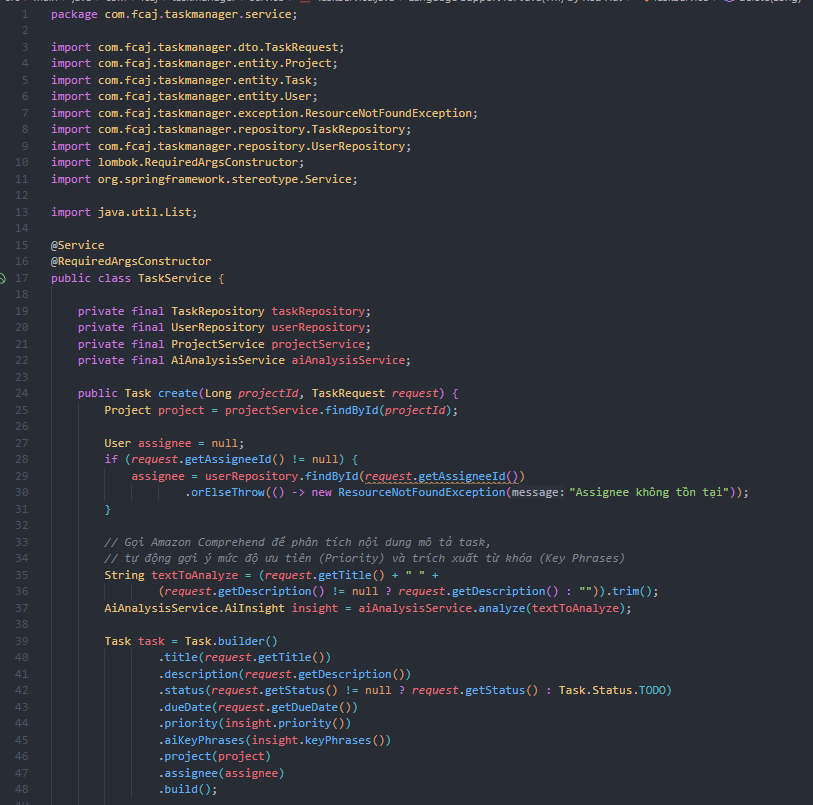
\includegraphics[width=10cm]{static/images/5-Workshop/5.10-TaskManager-AI/06-ai-priority-response.png}
        \caption{Response tạo task với \texttt{priority = HIGH} và \texttt{aiKeyPhrases} được điền tự động}
        \label{fig:ai-response}
    \end{figure}
\end{enumerate}

Đoạn mã dưới đây trích từ lớp \texttt{AiAnalysisService}, minh họa cách gọi
Amazon Comprehend và ánh xạ kết quả sentiment sang mức độ ưu tiên:

\begin{lstlisting}[style=javastyle, caption={Phân tích sentiment bằng Amazon Comprehend}, label={lst:comprehend}]
public AiInsight analyze(String text) {
    DetectSentimentRequest sentimentReq = DetectSentimentRequest.builder()
            .text(text)
            .languageCode(LanguageCode.VI)
            .build();
    DetectSentimentResponse sentimentRes = getClient().detectSentiment(sentimentReq);
    SentimentType sentiment = sentimentRes.sentiment();

    Task.Priority priority = mapSentimentToPriority(sentiment);
    return new AiInsight(priority, extractedKeyPhrases);
}
\end{lstlisting}

\textbf{Troubleshooting:} Một vấn đề gặp phải trong quá trình tích hợp AI --
task luôn được gợi ý \texttt{MEDIUM} dù mô tả mang sắc thái khẩn cấp; log
báo lỗi \texttt{The AWS Access Key Id needs a subscription for the service}
(HTTP 400). Nguyên nhân: Dịch vụ Amazon Comprehend chưa được kích hoạt trong
tài khoản ở region đang dùng. Giải pháp: Vào AWS Console → chọn đúng region
(\texttt{ap-southeast-1}) → tìm ``Comprehend'' → chạy thử \textbf{Real-time
analysis} một lần để kích hoạt (nằm trong Free Tier). Khi AI gọi lỗi, hệ
thống chủ động fallback về \texttt{MEDIUM} nên người dùng không gặp sự cố.

\subsubsection{Triển khai Frontend và kiểm thử end-to-end}

\begin{enumerate}[leftmargin=1.5cm]
    \item Sửa biến \texttt{API\_BASE} trong \texttt{frontend/js/config.js}
    thành địa chỉ EC2 thật (\texttt{http://<EC2-Public-IP>:8080}).

    \begin{figure}[H]
        \centering
        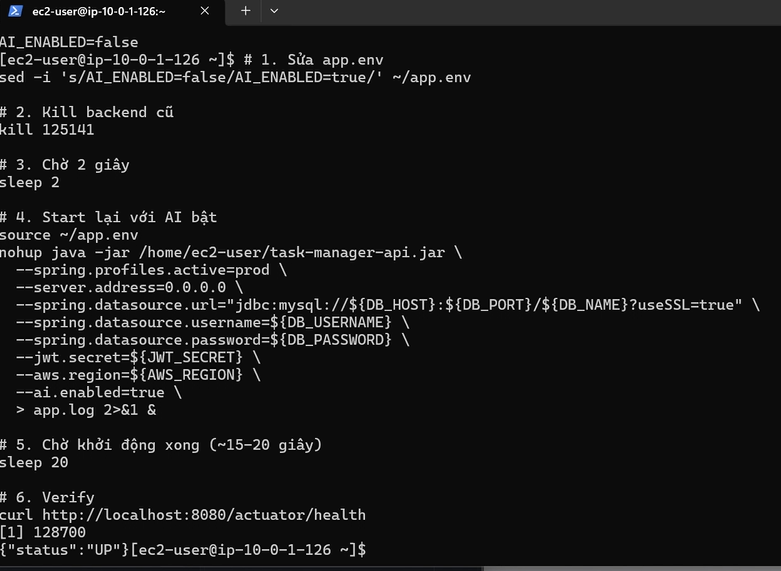
\includegraphics[width=10cm]{static/images/5-Workshop/5.11-TaskManager-Frontend/01-config-js.png}
        \caption{\texttt{API\_BASE} được đặt về địa chỉ public của EC2}
        \label{fig:frontend-config}
    \end{figure}

    \item Cài đặt Nginx trên EC2 (\texttt{sudo yum install -y nginx}), copy
    toàn bộ thư mục \texttt{frontend/} vào \texttt{/usr/share/nginx/html/},
    tạo server block trong \texttt{/etc/nginx/conf.d/taskmanager.conf} (listen
    \textbf{80}, \texttt{root /usr/share/nginx/html}, \texttt{try\_files \$uri
    \$uri/ /index.html;}).

    \begin{figure}[H]
        \centering
        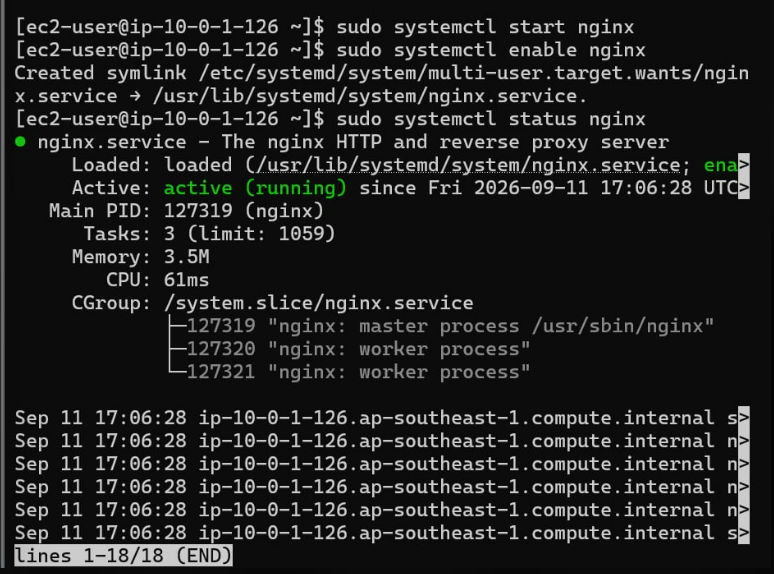
\includegraphics[width=10cm]{static/images/5-Workshop/5.11-TaskManager-Frontend/02-nginx-install.png}
        \caption{Nginx đã được cài trên EC2}
        \label{fig:nginx-install}
    \end{figure}

    \begin{figure}[H]
        \centering
        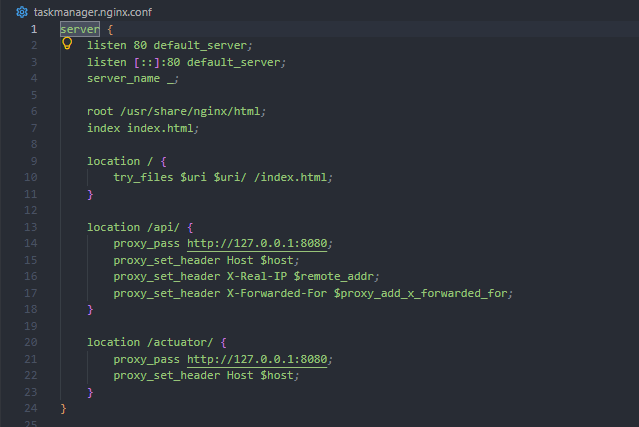
\includegraphics[width=10cm]{static/images/5-Workshop/5.11-TaskManager-Frontend/03-nginx-conf.png}
        \caption{Server block trong \texttt{taskmanager.conf}}
        \label{fig:nginx-conf}
    \end{figure}

    \item Khởi động và bật tự chạy: \texttt{sudo systemctl start nginx \&\&
    sudo systemctl enable nginx}. Mở \textbf{port 80} trong Security Group
    của EC2 (Custom TCP, source \texttt{0.0.0.0/0}).

    \begin{figure}[H]
        \centering
        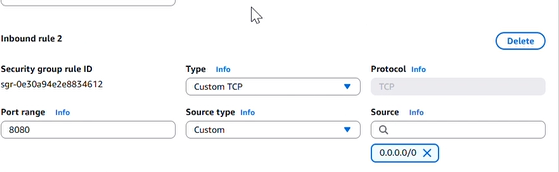
\includegraphics[width=10cm]{static/images/5-Workshop/5.11-TaskManager-Frontend/04-sg-port80.png}
        \caption{Port 80 mở cho HTTP trong Security Group của EC2}
        \label{fig:sg-port80}
    \end{figure}

    \item Truy cập qua \texttt{http://<EC2-Public-IP>}: đăng ký tài khoản
    mới, tạo project, tạo task với nhiều mức nội dung khác nhau để quan sát
    AI gợi ý priority khác nhau, đổi trạng thái task, xóa task/project.

    \begin{figure}[H]
        \centering
        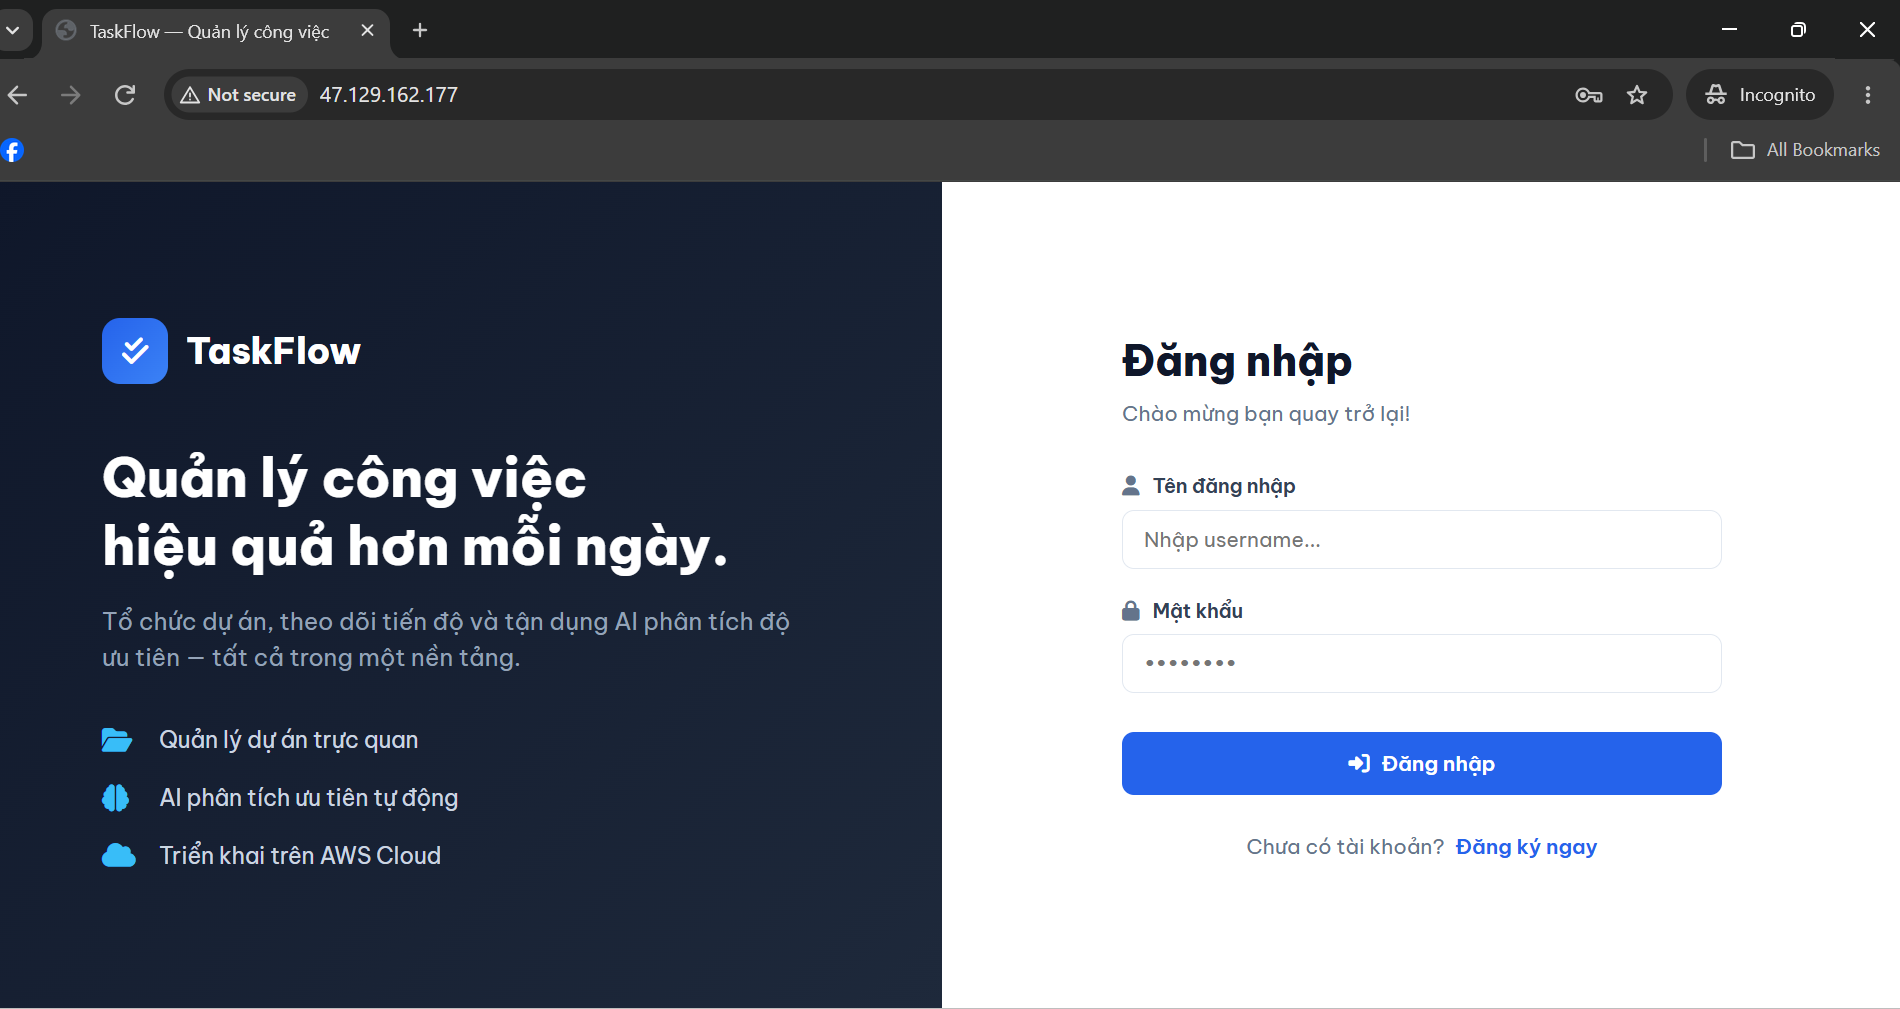
\includegraphics[width=10cm]{static/images/5-Workshop/5.11-TaskManager-Frontend/05-login-screen.png}
        \caption{Giao diện đăng nhập/đăng ký trên frontend}
        \label{fig:frontend-login}
    \end{figure}

    \begin{figure}[H]
        \centering
        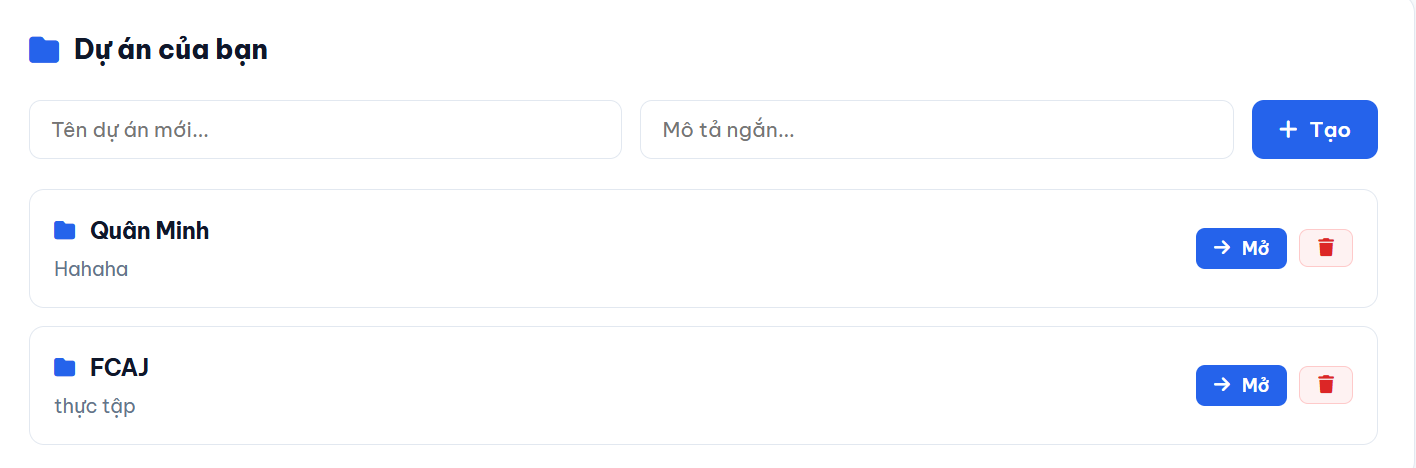
\includegraphics[width=10cm]{static/images/5-Workshop/5.11-TaskManager-Frontend/06-project-list.png}
        \caption{Danh sách project}
        \label{fig:frontend-projects}
    \end{figure}

    \begin{figure}[H]
        \centering
        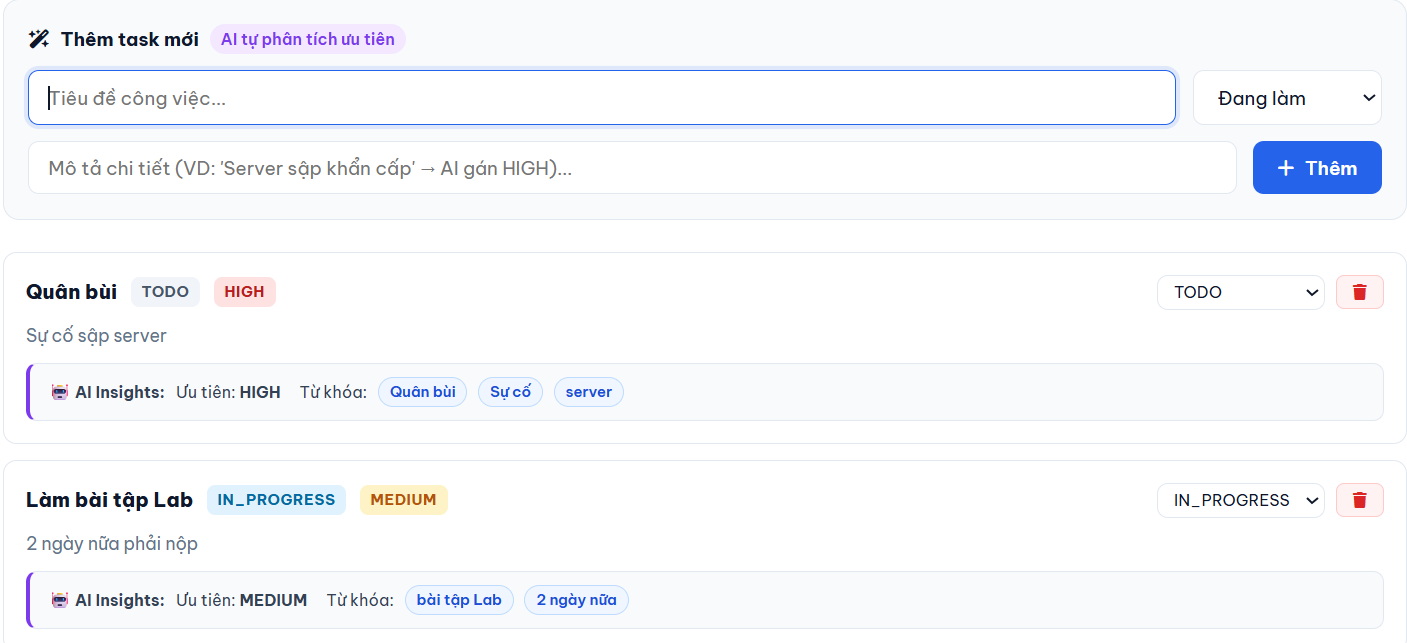
\includegraphics[width=10cm]{static/images/5-Workshop/5.11-TaskManager-Frontend/07-task-list-ai.png}
        \caption{Danh sách task hiển thị badge Priority và dòng ``AI nhận diện: ...''}
        \label{fig:frontend-tasks}
    \end{figure}
\end{enumerate}

\subsubsection{Chức năng của hệ thống}

Hệ thống đáp ứng đầy đủ quy trình quản lý công việc cơ bản. Người dùng có
thể đăng ký tài khoản mới, đăng nhập và nhận JWT token để sử dụng API. Trên
nền tảng đó, hệ thống hỗ trợ tạo, xem, cập nhật và xóa Project (CRUD
Project), cũng như tạo, xem, cập nhật và xóa Task trong từng Project (CRUD
Task). Mỗi Task có thể được cập nhật trạng thái TODO / IN\_PROGRESS / DONE
và gán cho một thành viên (assignee) cụ thể. Điểm nổi bật là tính năng
\textbf{tự động gợi ý mức độ ưu tiên (Priority) và trích xuất từ khóa bằng
AI (Amazon Comprehend)} mỗi khi tạo hoặc cập nhật task.

\textbf{Troubleshooting thường gặp khi triển khai Frontend:}
\begin{longtable}{p{5.5cm}p{8cm}}
\caption{Troubleshooting Frontend}
\label{tab:troubleshoot-frontend} \\
\toprule
\textbf{Vấn đề} & \textbf{Giải pháp} \\
\midrule
\endhead
Trang hiện ra nhưng CSS/JS không load (403) & Thư mục \texttt{css/}, \texttt{js/}
có quyền \texttt{dr-x------} (500) -- nginx không đọc được. Chạy \texttt{sudo
chmod 755} rồi \texttt{sudo chmod 644} cho các thư mục và file, restart nginx \\
Giao diện mất toàn bộ style, bố cục lỗi & File \texttt{style.css} bị lỗi cú
pháp (selector \texttt{.stat-label} thiếu dấu \texttt{\}}) làm trình duyệt bỏ
qua phần CSS phía sau. Đã sửa đúng và kiểm tra \\
Gọi API trả về 403 sau khi đổi JWT secret & Token cũ trong trình duyệt không
còn hợp lệ. Mở Console (F12) chạy \texttt{localStorage.clear()}, refresh
lại trang và đăng nhập mới \\
\bottomrule
\end{longtable}

\subsection{Dọn dẹp tài nguyên (Resource Cleanup)}

Để tránh phát sinh chi phí ngoài dự kiến sau khi hoàn thành thực tập, sinh
viên cần dọn dẹp toàn bộ tài nguyên đã tạo theo thứ tự:

\begin{enumerate}[leftmargin=1.5cm]
    \item \textbf{RDS}: Stop hoặc Delete instance \texttt{taskmanager-db}
    (lưu ý: Stop chỉ tạm dừng tối đa 7 ngày, sau đó AWS tự khởi động lại).
    \item \textbf{EC2}: Terminate các instance đã dùng cho workshop VPC và
    Task Manager API.
    \item \textbf{CloudFront + S3}: Disable rồi Delete Distribution, xóa
    nội dung và Delete bucket S3.
    \item \textbf{Lambda + API Gateway + DynamoDB}: Xóa Lambda function,
    xóa API Gateway, xóa bảng DynamoDB \texttt{fcaj-notes}.
    \item \textbf{IAM Role}: có thể giữ lại (không phát sinh phí) hoặc xóa
    nếu không còn dùng.
    \item Kiểm tra lại trang \textbf{Billing Dashboard} để xác nhận không
    còn tài nguyên nào phát sinh chi phí.
\end{enumerate}

\subsection{Kỹ năng và công cụ đã sử dụng}

Trong quá trình thực tập, sinh viên đã thực hành và củng cố nhiều kỹ năng
chuyên môn. Về phát triển backend, sinh viên thành thạo thiết kế và triển
khai REST API theo chuẩn RESTful, xác thực và phân quyền bằng JWT trong
Spring Security, cũng như thiết kế cơ sở dữ liệu quan hệ và ánh xạ
đối tượng-quan hệ (ORM) bằng Spring Data JPA/Hibernate. Trên hạ tầng AWS,
sinh viên biết cách triển khai ứng dụng lên EC2 và RDS theo mô hình mạng an
toàn (VPC 2-tier, Security Group, Private subnet cho database), tích hợp
dịch vụ AI (Amazon Comprehend) vào ứng dụng backend với quyền an toàn cấp
qua IAM Role thay vì hardcode credentials, đồng thời đóng gói ứng dụng bằng
Docker và quản lý đa container bằng Docker Compose. Ngoài ra, sinh viên còn
nắm được cách giám sát và kiểm soát chi phí dịch vụ cloud (AWS Budgets,
CloudWatch Billing Alarm), sử dụng Postman/curl để kiểm thử API, triển khai
frontend tĩnh lên EC2 bằng Nginx, và quản lý tài nguyên từ dòng lệnh với AWS
CLI.

\newpage

% ===================== PHẦN 4 =====================
\section{PHÂN TÍCH, ĐÁNH GIÁ VÀ ĐỀ XUẤT}

\subsection{Nhận xét về quy trình công việc}

Quy trình làm việc trong đợt thực tập tuân theo mô hình Agile tuần tự (iterative
incremental): mỗi tuần tương ứng một giai đoạn cụ thể với deliverable rõ ràng.
Tuần 1--3 tập trung vào việc làm quen nền tảng AWS và tích lũy kiến thức qua
các bài lab cơ bản. Tuần 4--5 bắt đầu triển khai các workshop thực hành độc lập
và thiết kế kiến trúc cho dự án chính. Tuần 6 là giai đoạn tích hợp và kiểm thử
toàn diện. Tuần 7 dành cho hoàn thiện báo cáo và nộp bài.

Các mốc quan trọng đều được hoàn thành đúng hạn: AWS Budget và CloudWatch
Billing Alarm được thiết lập trước khi chạy bất kỳ dịch vụ tốn phí nào (Tuần
4); hai workshop Static Website (S3 + CloudFront) và Serverless API (Lambda +
API Gateway + DynamoDB) hoàn thành ngay trong cùng tuần; backend Task Manager
Spring Boot triển khai thành công trên EC2 với JWT register hoạt động (Tuần
5); ca tích hợp Amazon Comprehend qua IAM Role thành công với priority gợi ý
đúng (Tuần 6); và toàn bộ hệ thống được kiểm thử end-to-end qua trình duyệt
cũng trong Tuần 6.

Tuy nhiên, cũng có một số trở ngại: việc kích hoạt Amazon Comprehend trong
tài khoản ở region \texttt{ap-southeast-1} mất thời gian tìm hiểu do lỗi
không rõ ràng (HTTP 400 thay vì lỗi quyền), và lỗi JWT\_SECRET quá ngắn
dẫn đến \texttt{SignatureException} -- cả hai đều được xử lý và ghi lại
trong tài liệu Troubleshooting.

\subsection{Khó khăn gặp phải và giải pháp}

Bảng \ref{tab:issues} tổng hợp một số khó khăn kỹ thuật tiêu biểu gặp phải
trong quá trình thực hiện dự án và hướng giải quyết tương ứng.

\begin{longtable}{p{5.5cm}p{8cm}}
\caption{Khó khăn và giải pháp}
\label{tab:issues} \\
\toprule
\textbf{Khó khăn} & \textbf{Giải pháp} \\
\midrule
\endhead
EC2 không kết nối được tới RDS &
Kiểm tra lại Security Group của RDS, bổ sung inbound rule cho phép port 3306
từ Security Group của EC2 (thay vì mở public). \\
CloudWatch Billing Alarm không hiển thị metric &
Bật tùy chọn ``Receive Billing Alerts'' trong Billing Preferences trước khi
tạo alarm; chuyển đúng region us-east-1. \\
Amazon Comprehend trả về HTTP 400 ``needs a subscription'' &
Kích hoạt dịch vụ Comprehend bằng cách chạy thử Real-time analysis một lần
trong đúng region (\texttt{ap-southeast-1}). \\
JWT\_SECRET quá ngắn gây ra SignatureException &
Đặt JWT\_SECRET tối thiểu 32 ký tự trong file \texttt{app.env}, restart service. \\
CSS/JS không load (403) trên Nginx &
Chỉnh quyền thư mục \texttt{css/}, \texttt{js/} thành 755/644, restart nginx. \\
Database chưa tồn tại khi RDS tạo mới &
Nếu ``Initial database name'' bỏ trống, cần tự tạo bằng lệnh SQL:
\texttt{CREATE DATABASE taskmanager;} qua MySQL client trên EC2. \\
\bottomrule
\end{longtable}

\subsection{Mối liên hệ giữa lý thuyết và thực tế}

Trong quá trình thực tập, các kiến thức đã học trên lớp được vận dụng rõ
ràng vào dự án thực tế. Kiến thức \textbf{mô hình quan hệ (Cơ sở dữ liệu)}
được áp dụng khi thiết kế 3 bảng users/projects/tasks với các ràng buộc khóa
ngoại (FK) và quan hệ 1--N, N--1. Kiến thức \textbf{giao thức HTTP/REST (Mạng
máy tính)} được dùng khi thiết kế REST API với các method GET, POST, PUT,
DELETE cùng mã trạng thái HTTP (200, 201, 400, 401, 403, 404). Kiến thức
\textbf{lập trình hướng đối tượng (Java)} thể hiện trong thiết kế các lớp
Entity, Repository, Service, Controller theo mô hình phân tầng của Spring
Boot. \textbf{Bảo mật ứng dụng} vận dụng kiến thức về mã hóa và quản lý phiên
qua BCrypt, JWT và phân quyền bằng Spring Security. Kiến thức \textbf{mạng
máy tính (VPC, Subnet, Routing)} về subnetting CIDR, routing table, Internet
Gateway được áp dụng trực tiếp khi thiết kế VPC 2-tier với public/private
subnet. Cuối cùng, \textbf{kiến trúc phần mềm} theo mô hình phân tầng
(presentation / application / data) được dùng trong kiến trúc 3 tầng
Frontend -- Backend -- Database của dự án.

\subsection{Đề xuất cải tiến}

Dự án còn nhiều hướng phát triển tiếp theo nếu có thêm thời gian. Ở tầng
bảo mật và hạ tầng, có thể bổ sung HTTPS cho backend thông qua Application
Load Balancer kết hợp AWS Certificate Manager, triển khai Auto Scaling Group
thay vì một EC2 đơn lẻ để tăng khả năng chịu tải, đồng thời đưa mật khẩu
database và JWT secret vào AWS Systems Manager Parameter Store thay vì biến
môi trường thô. Về quy trình phát triển, cần bổ sung CI/CD pipeline
(CodePipeline + CodeBuild) để tự động hóa quá trình triển khai cũng như thêm
unit test và integration test cho backend API. Cuối cùng, tính năng AI có
thể được mở rộng bằng cách huấn luyện mô hình riêng (ví dụ qua Amazon
SageMaker) để gợi ý priority chính xác hơn so với heuristic dựa trên
sentiment hiện tại, và bổ sung tính năng tóm tắt tự động nội dung task dài
bằng Amazon Bedrock.

\newpage

% ===================== PHẦN 5 =====================
\section{THAM GIA SỰ KIỆN VÀ BLOG KỸ THUẬT}

\subsection{Tham gia sự kiện: AWS Vietnam Community Meetup}

\textbf{Sự kiện:} AWS Vietnam Community Meetup -- Xu hướng AI \& Kiến trúc
Agentic trên AWS\\
\textbf{Thời gian:} Thứ Bảy, 25/07/2026 -- 08:30 đến 12:00\\
\textbf{Địa điểm:} AWS Hà Nội -- Tầng 7, Grand Terra Tower, 36 Cát Linh,
Đống Đa, Hà Nội\\
\textbf{Vai trò:} Người tham dự

Buổi meetup cộng đồng AWS nửa ngày quy tụ các AWS Community Hero, Community
Builder và kỹ sư đang trực tiếp triển khai AI trong doanh nghiệp. Chương
trình bao gồm 5 phiên:

\begin{longtable}{p{0.5cm}p{3cm}p{6cm}p{4cm}}
\caption{Chương trình AWS Vietnam Community Meetup}
\label{tab:meetup} \\
\toprule
\textbf{\#} & \textbf{Phiên} & \textbf{Nội dung} & \textbf{Diễn giả} \\
\midrule
\endhead
1 & Community Update & Cập nhật hoạt động cộng đồng AWS Việt Nam & Hồ Việt Anh, Phong Phạm \\
2 & OpenClaw & AI agent mã nguồn mở -- thiết lập, tích hợp tool, demo & Tuấn Vũ \\
3 & AI Trends $\rightarrow$ Business Value & Đặt AI trong khuôn khổ kết quả kinh doanh đo lường được & Nguyễn Thu, Nam La \\
4 & Ship Fast with AI & Dùng AI tăng tốc bàn giao, giữ human-in-the-loop & Henry (Đức) Bùi \\
5 & AI Agent Pattern on AWS & Khung quyết định chọn mẫu agent phù hợp trên AWS & Dũng Lương \\
\bottomrule
\end{longtable}

Buổi meetup mang lại cho sinh viên bốn bài học đáng giá. Thứ nhất, giá trị
của một AI agent nằm ở tầng tool và ngữ cảnh, không chỉ ở mô hình bên dưới.
Thứ hai, khi triển khai AI tại doanh nghiệp cần luôn gắn kết với kết quả
kinh doanh đo lường được, thay vì chỉ tập trung vào danh sách tính năng. Thứ
ba, human-in-the-loop là yêu cầu bắt buộc với mọi thứ chạm tới production.
Cuối cùng, nguyên tắc quan trọng là chọn mẫu agent đơn giản nhất giải quyết
được vấn đề, rồi mới tiến hóa thêm.

\subsection{Blog kỹ thuật: Guardrails trong Amazon Bedrock Knowledge Bases}

Sinh viên đã viết blog tổng hợp về Guardrails trong Amazon Bedrock Knowledge
Bases, trích xuất case study kiến trúc RAG Chatbot cho Enterprise trên AWS
Machine Learning Blog. Hệ thống được thiết kế theo tư duy Serverless với ba
thành phần trọng yếu. Thành phần đầu tiên là \textbf{tự động hóa Ingestion
\& Vector DB}: dữ liệu thô từ Amazon S3 được tự động phân tách, biến đổi
thành vector qua Amazon Bedrock Titan Embeddings và lưu trữ tại Amazon
OpenSearch Serverless. Thành phần thứ hai là \textbf{luồng xử lý trung tâm}:
Knowledge Bases for Amazon Bedrock đóng vai trò truy xuất ngữ cảnh và điều
phối câu hỏi sang Anthropic Claude 3 để tổng hợp phản hồi. Thành phần cuối
cùng là \textbf{kiểm soát rủi ro} khi tích hợp Bedrock Guardrails nhằm chặn
lọc các dữ liệu cá nhân nhạy cảm và giảm thiểu hiện tượng ảo giác của mô
hình LLM.

\textbf{Lợi ích:} Hệ thống đạt thời gian phản hồi dưới 2 giây mỗi truy
vấn; cắt giảm chi phí duy trì hạ tầng nhờ cơ chế On-Demand; Managed Services
giúp giản lược chi phí vận hành Vector Database thủ công.

\newpage

% ===================== PHẦN 6 =====================
\section{TỰ NHẬN XÉT VÀ ĐỊNH HƯỚNG NGHỀ NGHIỆP CÁ NHÂN}

\subsection{Tự đánh giá năng lực bản thân theo CLO}

\begin{longtable}{p{1.3cm}p{9cm}p{3cm}}
\caption{Sinh viên tự đánh giá theo từng CLO}
\label{tab:self-clo} \\
\toprule
\textbf{CLO} & \textbf{Minh chứng đạt được} & \textbf{Tự đánh giá (0--4)} \\
\midrule
\endhead
CLO1 & Phân tích được đặc điểm và phạm vi ứng dụng của 10 dịch vụ AWS đã sử
 dụng (S3, CloudFront, Lambda, API Gateway, DynamoDB, VPC, EC2, RDS,
Comprehend, IAM) &
3.5 \\
CLO2 & Thiết kế và triển khai hoàn chỉnh dự án Task Manager API (EC2 + RDS
trong VPC 2-tier), giải quyết trọn vẹn bài toán quản lý công việc nhỏ &
3.5 \\
CLO3 & Tích hợp thành công Amazon Comprehend vào Task Manager API để phân
 tích sentiment và gợi ý mức độ ưu tiên task tự động, không dùng hardcode
credentials &
3.5 \\
CLO4 & Hoàn thành đầy đủ Worklog 7 tuần, Blog kỹ thuật (Guardrails trong
Bedrock KB), bài thu hoạch sự kiện (AWS Community Meetup), và báo cáo
tổng kết này &
3.0 \\
CLO5 & Trao đổi thường xuyên với giảng viên hướng dẫn (\gvhd) và mentor
công ty (\mentorCT) trong suốt quá trình thực tập &
3.0 \\
\bottomrule
\end{longtable}

\subsection{Điểm mạnh và điểm cần cải thiện}

Qua đợt thực tập, sinh viên nhận thấy bản thân có những điểm mạnh nổi bật.
Đó là khả năng tự học công nghệ mới: chỉ trong 7 tuần, sinh viên đã làm quen
và triển khai được 10+ dịch vụ AWS, từ cơ bản (EC2, S3) đến nâng cao (VPC
2-tier, IAM Role, Comprehend). Điểm mạnh thứ hai là tư duy triển khai
end-to-end: từ thiết kế kiến trúc, viết mã nguồn, cấu hình hạ tầng, tích hợp
AI, đến triển khai và kiểm thử toàn diện. Bên cạnh đó, kỹ năng giao tiếp và
viết tài liệu được thể hiện qua Worklog chi tiết theo từng ngày, blog kỹ
thuật và báo cáo có cấu trúc rõ ràng. Cuối cùng, sinh viên áp dụng tốt thực
hành bảo mật khi dùng JWT + BCrypt, đưa database vào private subnet và dùng
IAM Role thay vì key tĩnh.

Ngược lại, sinh viên xác định một số điểm cần cải thiện. Kinh nghiệm xử lý
sự cố production còn hạn chế -- một số lỗi (Comprehend chưa activated,
JWT\_SECRET quá ngắn) mất thời gian tìm hiểu hơn mức cần thiết. Kiến thức
bảo mật nâng cao cần được mở rộng thêm, ví dụ chứng thực HTTPS cho backend,
secrets management (SSM Parameter Store) và VPC endpoints. Ngoài ra, tính kỷ
luật trong việc tuân thủ lịch trình cần được nâng cao hơn -- một số task bị
trễ do dành quá nhiều thời gian cho troubleshooting.

\subsection{Kế hoạch phát triển nghề nghiệp}

Sau khi tốt nghiệp, em định hướng ứng tuyển vị trí \textbf{Java Backend
Developer}, tập trung vào mảng phát triển ứng dụng trên hạ tầng cloud. Để
đạt được định hướng đó, em dự kiến tìm hiểu sâu hơn về microservices
architecture, container orchestration (Kubernetes) và service mesh; chuẩn bị
chứng chỉ \textbf{AWS Certified Developer -- Associate} nhằm chuẩn hóa kiến
thức AWS đã tích lũy; tiếp tục phát triển portfolio với các dự án backend
cloud-native, tích hợp AI/ML services; đồng thời nâng cao kỹ năng DevOps với
CI/CD pipeline, Infrastructure as Code (Terraform/CloudFormation) cùng
monitoring và observability.

\newpage

% ===================== PHẦN 7 =====================
\section{KẾT LUẬN VÀ KIẾN NGHỊ}

\subsection{Kết luận}

Qua 7 tuần thực tập tốt nghiệp tại chương trình FCAJ (First Cloud AI Journey)
của Công ty TNHH Amazon Web Services Việt Nam, em đã hoàn thành toàn bộ nội
dung thực hành theo kế hoạch đề ra. Cụ thể, em đã hoàn thành khóa học nền
tảng AWS cùng 4 workshop thực hành gồm giám sát chi phí (Budgets +
CloudWatch), website tĩnh (S3 + CloudFront), Serverless API (Lambda + API
Gateway + DynamoDB) và thiết kế mạng VPC 2-tier. Trên nền tảng đó, em xây
dựng và triển khai thành công dự án \textbf{Task Manager API} -- một hệ
thống backend hoàn chỉnh theo mô hình EC2 + RDS trên AWS, kết hợp công nghệ
Java Spring Boot 3.3, đồng thời tích hợp thành công \textbf{Amazon
Comprehend} (AI/NLP) để tự động phân tích sentiment và gợi ý mức độ ưu tiên
task -- đáp ứng CLO3 của học phần. Em cũng hoàn tất việc triển khai frontend
lên EC2 với Nginx và kiểm thử end-to-end toàn bộ hệ thống, tham gia sự kiện
AWS Vietnam Community Meetup, viết blog kỹ thuật về Guardrails trong Amazon
Bedrock Knowledge Bases, và deploy website báo cáo thực tập lên GitHub Pages
bằng Hugo.

Đợt thực tập đã giúp em củng cố kiến thức về điện toán đám mây, phát triển
backend, tích hợp AI, và tích lũy kinh nghiệm thực tế trong việc triển khai
một ứng dụng từ giai đoạn thiết kế tới vận hành trên hạ tầng cloud thật.

\subsection{Kiến nghị}

Từ trải nghiệm thực tế, em có một số đề xuất. Thứ nhất, Nhà trường/Khoa nên
tăng thời lượng thực hành AWS Cloud trong chương trình đào tạo, vì đây là kỹ
năng ngày càng quan trọng trong ngành phát triển phần mềm. Thứ hai, Khoa nên
bổ sung tài liệu hướng dẫn về bảo mật cloud (IAM best practices, VPC design
patterns) làm tài liệu tham khảo cho sinh viên thực tập. Cuối cùng, em đề
xuất chương trình FCAJ mở rộng thời gian thực tập (ví dụ 8--10 tuần) để sinh
viên có thêm thời gian hoàn thiện dự án và viết báo cáo chất lượng hơn.

\newpage

% ===================== TÀI LIỆU THAM KHẢO =====================
\section*{TÀI LIỆU THAM KHẢO}
\addcontentsline{toc}{section}{TÀI LIỆU THAM KHẢO}

\begin{enumerate}[leftmargin=1.5cm]
    \item Amazon Web Services, \textit{AWS Documentation},
    \url{https://docs.aws.amazon.com}
    \item Spring Framework, \textit{Spring Boot Reference Documentation},
    \url{https://docs.spring.io/spring-boot/}
    \item Amazon Web Services, \textit{Amazon Comprehend Developer Guide},
    \url{https://docs.aws.amazon.com/comprehend/}
    \item AWS Study Group, \textit{FCAJ -- First Cloud AI Journey},
    \url{https://cloudjourney.awsstudygroup.com/}
    \item Trường Đại học Xây dựng Hà Nội, \textit{Quy định Tổ chức và Đánh
    giá Thực tập tốt nghiệp}, ban hành kèm Quyết định số
    /QĐ-ĐHXDHN.
    \item Khoa Công nghệ Thông tin, Trường Đại học Xây dựng Hà Nội,
    \textit{Đề cương chi tiết học phần Thực tập tốt nghiệp} (mã học phần
    608821).
    \item Amazon Web Services, \textit{Introducing Guardrails in Knowledge
    Bases for Amazon Bedrock},
    \url{https://aws.amazon.com/blogs/machine-learning/introducing-guardrails-in-knowledge-bases-for-amazon-bedrock/}
\end{enumerate}

\newpage

% ===================== PHỤ LỤC =====================
\section*{PHỤ LỤC}
\addcontentsline{toc}{section}{PHỤ LỤC}

\subsection*{Phụ lục A: Mã nguồn chính -- AiAnalysisService}

Trích từ lớp \texttt{AiAnalysisService} trong dự án Task Manager API, thể
hiện cách gọi Amazon Comprehend và ánh xạ sentiment sang mức độ ưu tiên task:

\begin{lstlisting}[style=javastyle, caption={AiAnalysisService -- Gọi Comprehend và gợi ý Priority}, label={lst:ai-service}]
@Service
public class AiAnalysisService {

    private final ComprehendClient client;

    public AiInsight analyze(String text) {
        // 1. Phân tích sentiment
        DetectSentimentRequest sentimentReq = DetectSentimentRequest.builder()
                .text(text)
                .languageCode(LanguageCode.VI)
                .build();
        DetectSentimentResponse sentimentRes =
                getClient().detectSentiment(sentimentReq);
        SentimentType sentiment = sentimentRes.sentiment();

        // 2. Trích xuất key phrases
        DetectKeyPhrasesRequest kpReq = DetectKeyPhrasesRequest.builder()
                .text(text)
                .languageCode(LanguageCode.VI)
                .build();
        DetectKeyPhrasesResponse kpRes = getClient().detectKeyPhrases(kpReq);
        List<String> keyPhrases = kpRes.keyPhrases().stream()
                .map(KeyPhrase::text)
                .collect(Collectors.toList());

        // 3. Ánh xạ sentiment -> Priority
        Task.Priority priority = mapSentimentToPriority(sentiment);
        return new AiInsight(priority, String.join(", ", keyPhrases));
    }

    private Task.Priority mapSentimentToPriority(SentimentType sentiment) {
        return switch (sentiment) {
            case NEGATIVE, VERY_NEGATIVE -> Task.Priority.HIGH;
            case NEUTRAL -> Task.Priority.MEDIUM;
            case POSITIVE, VERY_POSITIVE -> Task.Priority.LOW;
        };
    }
}
\end{lstlisting}

\subsection*{Phụ lục B: Bảng Worklog chi tiết 7 tuần}

\begin{longtable}{p{1.5cm}p{2.5cm}p{10cm}}
\caption{Worklog chi tiết thực tập}
\label{tab:worklog} \\
\toprule
\textbf{Tuần} & \textbf{Thời gian} & \textbf{Nội dung chính} \\
\midrule
\endhead
1 & 25/07--31/07/2026 & Giới thiệu công ty AWS VN; tạo tài khoản AWS Free
Tier với MFA; khám phá AWS Console; tìm hiểu các nhóm dịch vụ Compute,
Storage, Networking, Database \\
2 & 01/08--07/08/2026 & Học EC2 (AMI, EBS, Security Group); lab khởi chạy
EC2 + SSH; học VPC (subnet, route table, IGW); lab tạo VPC tùy chỉnh và
triển khai ứng dụng web trên EC2 \\
3 & 08/08--14/08/2026 & Học S3 (versioning, lifecycle); thực hành DynamoDB
(tạo bảng, query); cấu hình S3 versioning; CloudWatch (metrics, alarm,
dashboard); cài đặt AWS CLI \\
4 & 15/08--21/08/2026 & AWS Budget (\texttt{FCAJ-Budget}, 5 USD) + CloudWatch
Billing Alarm; Workshop Static Website (S3 + CloudFront HTTPS); Workshop
Serverless API (Lambda + API GW + DynamoDB); kiểm thử GET/POST \\
5 & 22/08--28/08/2026 & VPC 2-tier (public/private subnet); khởi chạy EC2
+ SSH; thiết kế DB Task Manager; RDS MySQL private; deploy backend Spring
Boot trên EC2; JWT register test \\
6 & 29/08--04/09/2026 & IAM Role \texttt{ComprehendReadOnly} + gắn EC2;
tích hợp Amazon Comprehend (AI priority); deploy frontend (Nginx on EC2);
E2E test (CRUD + AI); hướng dẫn cleanup \\
7 & 05/09--08/09/2026 & Fork Hugo template; tùy chỉnh config; điền nội
dung worklog/workshop; cấu hình GitHub Actions deploy; viết tự đánh giá,
phản hồi, bài thu hoạch sự kiện; đọc soát và nộp báo cáo \\
\bottomrule
\end{longtable}

\subsection*{Phụ lục C: Danh mục hình ảnh minh chứng}

Bảng dưới đây liệt kê tất cả ảnh chụp màn hình được sử dụng trong báo cáo,
đã lưu tại thư mục \texttt{static/images/5-Workshop/} theo từng mục workshop.

\begin{longtable}{p{5.5cm}p{8cm}}
\caption{Danh mục ảnh minh chứng các workshop}
\label{tab:images} \\
\toprule
\textbf{Workshop} & \textbf{File ảnh} \\
\midrule
\endhead
5.2 Environment Setup & \texttt{01-console-login.png}, \texttt{02-region-selector.png}, \texttt{03-region-confirmed.png} \\
5.3 Cost Monitoring & \texttt{01-budget-menu.png} -- \texttt{07-subscription-email.png} (7 ảnh) \\
5.4 S3 + CloudFront & \texttt{02-create-bucket.png} -- \texttt{09-site-https.png} (8 ảnh) \\
5.5 Serverless API & \texttt{02-dynamodb-create-table.png} -- \texttt{11-postman-post.png} (10 ảnh) \\
5.6 VPC 2-tier & \texttt{02-create-vpc.png} -- \texttt{10-ssh-success.png} (9 ảnh) \\
5.8 Task Manager RDS & \texttt{01-rds-create.png}, \texttt{02-rds-config.png}, \texttt{03-rds-available.png} \\
5.9 Task Manager EC2 & \texttt{01-ec2-launch.png} -- \texttt{06-register-jwt.png} (6 ảnh) \\
5.10 Task Manager AI & \texttt{01-iam-create-role.png} -- \texttt{06-ai-priority-response.png} (6 ảnh) \\
5.11 Task Manager Frontend & \texttt{01-config-js.png} -- \texttt{07-task-list-ai.png} (7 ảnh) \\
\bottomrule
\end{longtable}

\end{document}
